\documentclass[a4paper,12pt]{report}

% ==================================================
% PACKAGES
% ==================================================

\usepackage[T1]{fontenc}
\usepackage[utf8]{inputenc}
\usepackage[french]{babel}

\usepackage{array}
\usepackage{longtable}
\usepackage{graphicx}
\usepackage{booktabs}
\usepackage{float}
\usepackage{titlesec}
\usepackage{minitoc}
\usepackage{caption}

\usepackage[
left=2.5cm,
right=2.5cm,
top=2.5cm,
bottom=2.5cm
]{geometry}

\usepackage{fancyhdr}

% ==================================================
% HEADER & FOOTER
% ==================================================

\pagestyle{fancy}

\fancyhf{}

\fancyhead[L]{\nouppercase{\leftmark}}

\fancyfoot[C]{\thepage}

\renewcommand{\headrulewidth}{0.4pt}

\setlength{\headheight}{15pt}

% ==================================================
% CONFIGURATION
% ==================================================

\dominitoc

% ==================================================
% RACCOURCIR L'INTRODUCTION GENERALE
% ==================================================

% Réduction de l'interligne pour l'introduction générale
\newcommand{\introspacing}{%
\renewcommand{\baselinestretch}{0.9}\normalsize%
}

% ==================================================
% DOCUMENT
% ==================================================

\begin{document}

% ==================================================
% PAGE DE GARDE
% ==================================================

\begin{titlepage}

\centering

\vspace*{1.5cm}

{\Huge \textbf{Rapport de Projet de Fin d'Études}}

\vspace{1.5cm}

{\LARGE \textbf{Maison3D Immobilier}}

\vspace{0.5cm}

{\Large Plateforme web intelligente de gestion immobilière}

\vspace{2cm}

% ==================================================
% LOGO - Version avec vérification d'existence
% ==================================================

\IfFileExists{images/we_are_tech.jpg}{%
    \begin{figure}[H]
    \centering
    
\includegraphics[width=5cm]{images/we_are_tech.jpg}
    \caption*{Logo de l'entreprise We Are Tech}
    \end{figure}
}{%
    \begin{figure}[H]
    \centering
    \fbox{\begin{minipage}{5cm}
    \centering
    \vspace{2cm}
    \textbf{Logo We Are Tech}
    \vspace{2cm}
    \end{minipage}}
    \caption*{Logo de l'entreprise We Are Tech (à insérer)}
    \end{figure}
}

\vspace{1cm}

\begin{flushleft}

\textbf{Réalisé par :} Montassar Gassara

\vspace{0.4cm}

\textbf{Encadrant académique :} [Nom Encadrant]

\vspace{0.4cm}

\textbf{Encadrant professionnel :} [Nom Encadrant]

\vspace{0.4cm}

\textbf{Entreprise :} We Are Tech

\vspace{0.4cm}

\textbf{Année universitaire :} 2025-2026

\end{flushleft}

\vfill

\end{titlepage}

% ==================================================
% REMERCIEMENTS
% ==================================================

\chapter*{Remerciements}

\addcontentsline{toc}{chapter}{Remerciements}

Avant tout développement de ce projet, je tiens à adresser mes sincères remerciements à toutes les personnes ayant contribué à la réalisation de ce travail dans les meilleures conditions.

J'exprime ma profonde gratitude à l'entreprise \textbf{We Are Tech} pour m'avoir accueilli durant cette période de stage et pour m'avoir offert un environnement professionnel motivant et enrichissant.

Je remercie particulièrement mon encadrant professionnel pour son accompagnement, ses conseils précieux ainsi que son soutien tout au long du projet.

J'adresse également mes remerciements à mon encadrant académique pour son suivi, ses orientations et ses recommandations qui ont contribué à la réussite de ce travail.

Enfin, je remercie toutes les personnes ayant participé de près ou de loin à la réalisation de ce projet.

\newpage

% ==================================================
% TABLE DES MATIERES
% ==================================================

\tableofcontents

\newpage

% ==================================================
% LISTE DES FIGURES
% ==================================================

\listoffigures

\newpage

% ==================================================
% LISTE DES TABLEAUX
% ==================================================

\listoftables

\newpage

% ==================================================
% INTRODUCTION GENERALE (VERSION SUR UNE PAGE)
% ==================================================

\chapter*{Introduction générale}

\addcontentsline{toc}{chapter}{Introduction générale}

\begingroup
\introspacing

La transformation numérique connaît aujourd'hui une évolution rapide dans plusieurs secteurs d'activité, notamment dans le domaine immobilier. Les agences immobilières recherchent désormais des solutions digitales modernes capables de centraliser la gestion des biens, d'améliorer la communication interne et d'optimiser les processus de vente et de location.

Cependant, plusieurs agences utilisent encore des outils classiques ou des plateformes limitées ne répondant pas aux exigences actuelles du marché immobilier. L'utilisation des fichiers Excel, des systèmes manuels ou des applications non centralisées entraîne plusieurs problèmes tels que la perte de temps, les difficultés de collaboration, le manque de suivi des transactions ainsi que l'absence de gestion intelligente des utilisateurs et des rôles.

Dans ce contexte, mon projet de fin d'études intitulé \textbf{Maison3D Immobilier} consiste à concevoir et développer une plateforme web immobilière intelligente permettant la gestion centralisée des agences immobilières, des biens immobiliers, des transactions, des affiliations et des communications internes.

La plateforme repose sur une architecture moderne basée sur les technologies \textbf{Angular} pour la partie frontend et \textbf{Spring Boot} pour la partie backend. Elle intègre également un système de sécurité basé sur l'authentification JWT ainsi qu'une gestion hiérarchique des rôles permettant d'adapter les fonctionnalités selon chaque type d'utilisateur.

Le système propose plusieurs fonctionnalités importantes telles que :

\begin{itemize}
\item la gestion des agences immobilières ;
\item la gestion des biens immobiliers ;
\item la gestion des ventes et des locations ;
\item la gestion des affiliés et des commissions ;
\item la gestion des utilisateurs et des rôles ;
\item les dashboards intelligents ;
\item la messagerie interne en temps réel ;
\item la gestion des contrats et renouvellements ;
\item les statistiques et indicateurs de performance.
\end{itemize}

L'objectif principal du projet est de développer une plateforme professionnelle, moderne, sécurisée et évolutive répondant aux besoins réels des agences immobilières tout en améliorant la productivité, l'organisation interne et l'expérience utilisateur.

Ce rapport est organisé en plusieurs chapitres :

\begin{itemize}
\item Un premier chapitre intitulé \textit{Présentation générale du projet} présente l'organisme d'accueil, le contexte général du projet, l'étude de l'existant ainsi que la méthodologie de développement adoptée.

\item Un deuxième chapitre intitulé \textit{Initiation du projet et étude technique} présente les besoins fonctionnels et non fonctionnels, les différents acteurs du système, l'architecture globale ainsi que les technologies utilisées.

\item Les chapitres suivants présenteront les différents sprints réalisés durant le développement de la plateforme à travers l'analyse, la conception UML ainsi que la réalisation des différentes fonctionnalités du système.
\end{itemize}

\endgroup

% ==================================================
% CHAPITRE 1
% ==================================================

\chapter{Présentation générale du projet}

\minitoc

% ==================================================
% INTRODUCTION
% ==================================================

\section{Introduction}

Dans ce premier chapitre, je présente le cadre général du projet afin d'avoir une vision globale sur le système développé ainsi que son environnement de réalisation.

Je commence par présenter l'organisme d'accueil dans lequel le projet a été réalisé. Ensuite, je présente le contexte général du projet ainsi que les problèmes rencontrés dans le domaine immobilier moderne. J'expose également l'étude de l'existant, les limites des solutions actuelles ainsi que la solution proposée.

Enfin, je présente la méthodologie de développement adoptée pour la réalisation du projet.

% ==================================================
% ENTREPRISE
% ==================================================

\section{Présentation de l'organisme d'accueil}

Le projet de fin d'études a été réalisé au sein de la société \textbf{We Are Tech}, une entreprise spécialisée dans le développement des solutions digitales innovantes et des applications web modernes.

La société accompagne différentes entreprises dans leur transformation numérique à travers la conception et le développement d'applications performantes, sécurisées et évolutives répondant aux besoins des clients.

We Are Tech intervient dans plusieurs domaines technologiques tels que :

\begin{itemize}
\item le développement web ;
\item le développement mobile ;
\item le marketing digital ;
\item l'optimisation SEO ;
\item les solutions Cloud ;
\item la création de contenu numérique.
\end{itemize}

L'entreprise utilise plusieurs technologies modernes parmi lesquelles :

\begin{itemize}
\item Angular ;
\item Spring Boot ;
\item React Native ;
\item MySQL ;
\item Docker ;
\item GitHub ;
\item les solutions Cloud.
\end{itemize}

Grâce à une organisation collaborative et une équipe multidisciplinaire, We Are Tech assure la réalisation de solutions numériques adaptées aux besoins des clients tout en garantissant la qualité et la maintenabilité des projets développés.

\begin{figure}[H]
\centering
\IfFileExists{images/we_are_tech.jpg}{%
    
\includegraphics[width=6cm]{images/we_are_tech.jpg}
}{%
    \fbox{\begin{minipage}{6cm}
    \centering
    \vspace{2.5cm}
    \textbf{Logo We Are Tech}
    \vspace{2.5cm}
    \end{minipage}}
}
\caption{Logo de l'entreprise We Are Tech}
\end{figure}

% ==================================================
% PRESENTATION PROJET
% ==================================================

\section{Présentation du projet}

Le projet intitulé \textbf{Maison3D Immobilier} s'inscrit dans le cadre du projet de fin d'études réalisé pour conclure ma formation universitaire.

L'objectif principal du projet consiste à développer une plateforme web immobilière moderne permettant aux agences immobilières de gérer efficacement leurs biens, leurs transactions, leurs utilisateurs ainsi que leurs communications internes.

La plateforme permet également de centraliser plusieurs opérations importantes telles que :

\begin{itemize}
\item la gestion des biens immobiliers ;
\item la gestion des ventes et locations ;
\item la gestion des agences ;
\item la gestion des commerciaux ;
\item la gestion des affiliés ;
\item la gestion des commissions ;
\item les dashboards intelligents ;
\item la communication interne en temps réel.
\end{itemize}

Le système repose sur une architecture moderne basée sur Angular et Spring Boot afin de garantir la performance, la sécurité et l'évolutivité de l'application.

% ==================================================
% ETUDE EXISTANT
% ==================================================

\section{Étude de l'existant}

\subsection{Analyse de l'existant}

Actuellement, plusieurs plateformes immobilières existent sur le marché et proposent des services de publication et de gestion des annonces immobilières.

\subsubsection{Plateforme Properstar}

\textbf{Properstar} est une plateforme immobilière internationale permettant la consultation et la publication d'annonces immobilières dans plusieurs pays.

La plateforme propose plusieurs fonctionnalités telles que :

\begin{itemize}
\item recherche avancée des biens immobiliers ;
\item filtrage par prix, localisation et catégorie ;
\item consultation des détails des propriétés ;
\item affichage des images des biens ;
\item contact avec les agences immobilières.
\end{itemize}

Cependant, Properstar présente certaines limites dans le cadre de la gestion interne des agences immobilières :

\begin{itemize}
\item absence de gestion hiérarchique des rôles ;
\item absence de messagerie interne professionnelle ;
\item manque de gestion des affiliations ;
\item absence de dashboard intelligent personnalisé ;
\item absence de gestion avancée des commissions.
\end{itemize}

\begin{figure}[H]
\centering
\IfFileExists{images/Properstar.png}{%
    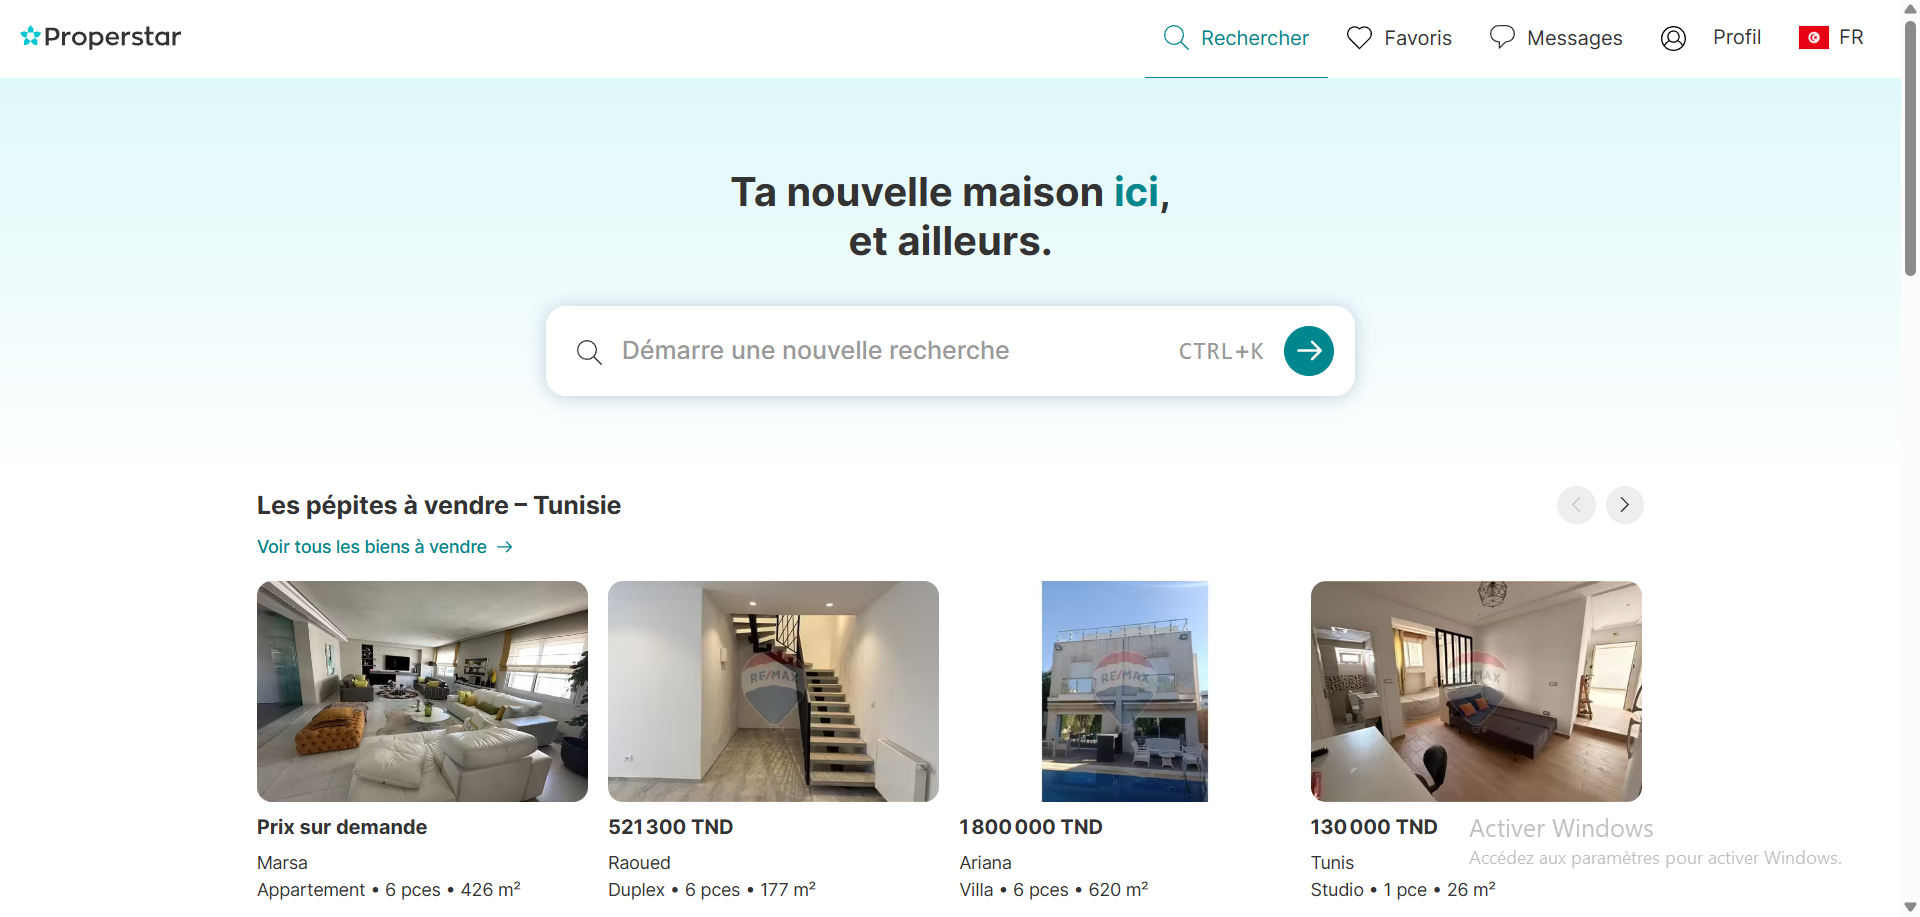
\includegraphics[width=12cm]{images/Properstar.png}
}{%
    \fbox{\begin{minipage}{10cm}
    \centering
    \vspace{3cm}
    \textit{Capture d'écran Properstar (à insérer)}
    \vspace{3cm}
    \end{minipage}}
}
\caption{Interface de la plateforme Properstar}
\end{figure}

% ==================================================
% MUBAWAB
% ==================================================

\subsubsection{Plateforme Mubawab}

\textbf{Mubawab} est une plateforme spécialisée dans les annonces immobilières permettant la vente et la location des biens immobiliers.

Elle offre plusieurs fonctionnalités importantes :

\begin{itemize}
\item publication des annonces immobilières ;
\item consultation des biens disponibles ;
\item système de recherche immobilière ;
\item affichage des informations détaillées ;
\item contact entre clients et agences.
\end{itemize}

Malgré ses avantages, plusieurs limitations ont été identifiées :

\begin{itemize}
\item absence d'une gestion complète des agences ;
\item absence de communication interne temps réel ;
\item absence de gestion avancée des utilisateurs ;
\item manque de statistiques intelligentes ;
\item absence de gestion des contrats et renouvellements.
\end{itemize}

\begin{figure}[H]
\centering
\IfFileExists{images/mubawab.png}{%
    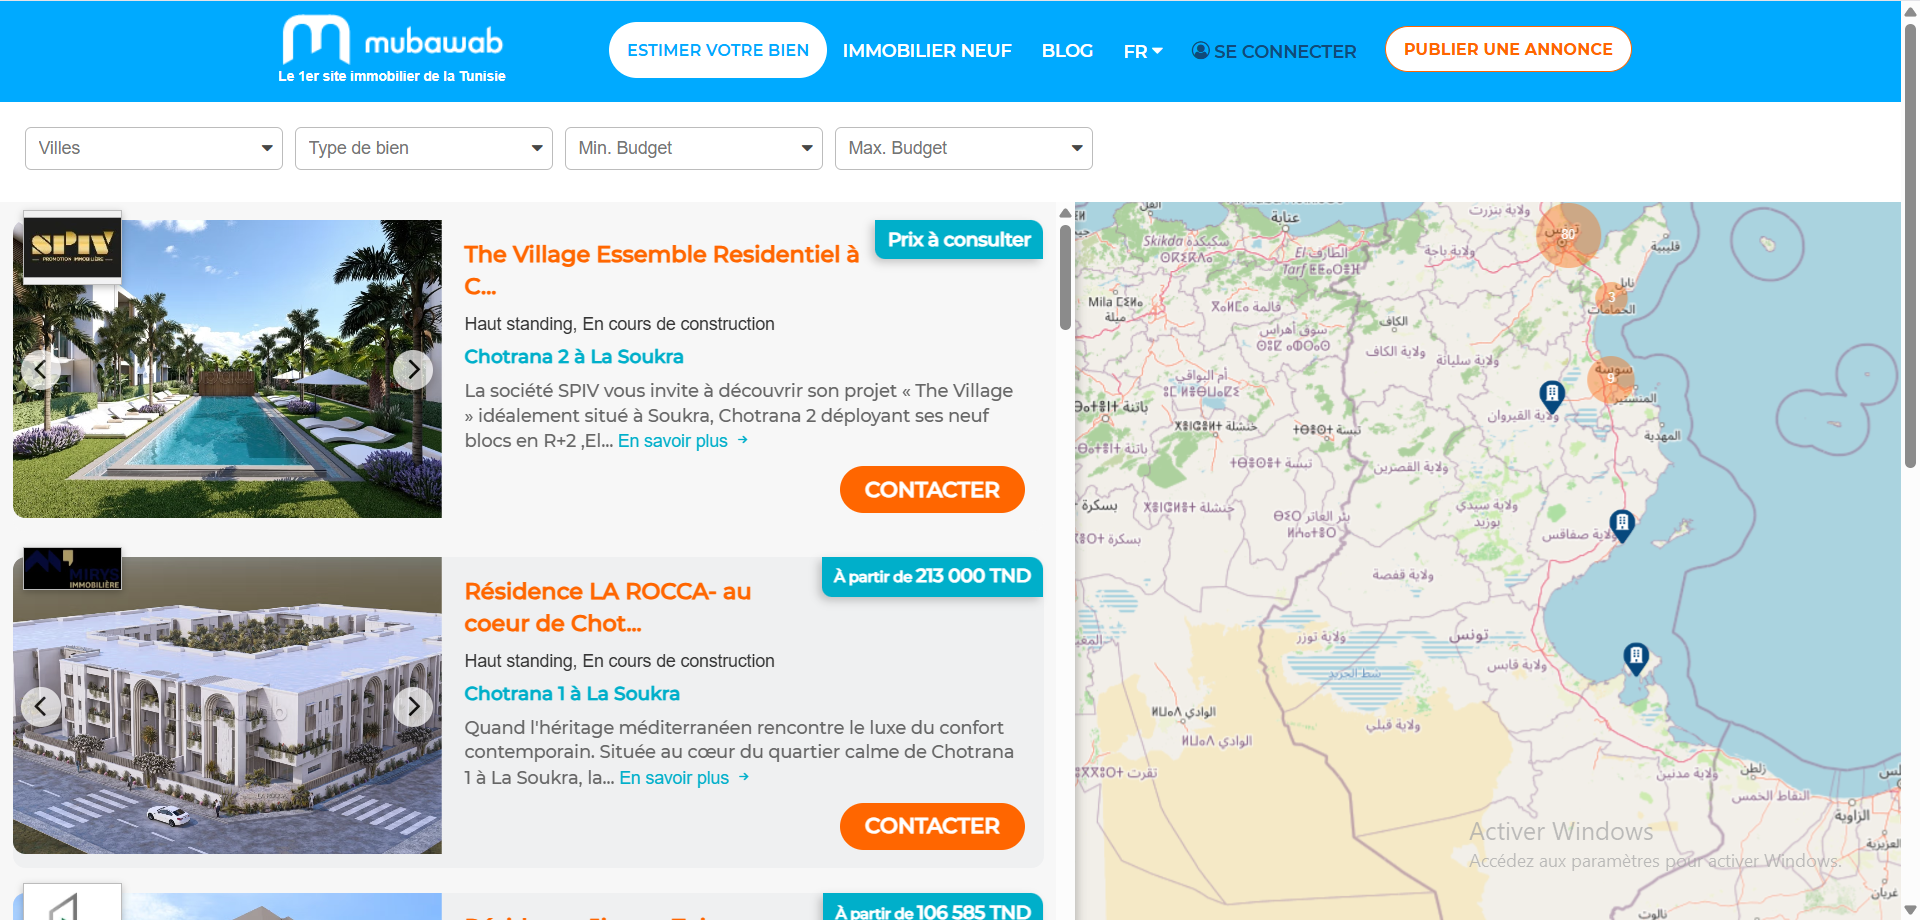
\includegraphics[width=12cm]{images/mubawab.png}
}{%
    \fbox{\begin{minipage}{10cm}
    \centering
    \vspace{3cm}
    \textit{Capture d'écran Mubawab (à insérer)}
    \vspace{3cm}
    \end{minipage}}
}
\caption{Interface de la plateforme Mubawab}
\end{figure}

% ==================================================
% GESTION MANUELLE
% ==================================================

\subsubsection{Gestion manuelle}

Certaines agences utilisent encore des outils classiques tels que les fichiers Excel, les documents papier ou des systèmes non centralisés.

Cette méthode présente plusieurs inconvénients :

\begin{itemize}
\item absence de centralisation des données ;
\item risque élevé d'erreurs ;
\item difficulté de collaboration ;
\item manque de sécurité ;
\item perte de temps dans les opérations.
\end{itemize}

% ==================================================
% CRITIQUE EXISTANT
% ==================================================

\subsection{Critique de l'existant}

L'analyse des solutions existantes a permis d'identifier plusieurs insuffisances :

\begin{itemize}
\item absence d'une plateforme centralisée ;
\item manque de gestion hiérarchique des rôles ;
\item absence de gestion des affiliations ;
\item absence de communication interne intégrée ;
\item manque de dashboards intelligents ;
\item limitations dans le suivi des transactions ;
\item absence de gestion avancée des commissions ;
\item sécurité limitée dans certaines solutions.
\end{itemize}

% ==================================================
% SOLUTION PROPOSEE
% ==================================================

\section{Solution proposée}

Afin de répondre aux limites identifiées dans les solutions existantes, je propose une plateforme web immobilière moderne appelée \textbf{Maison3D Immobilier}.

Cette plateforme permet :

\begin{itemize}
\item la centralisation des opérations immobilières ;
\item la gestion des agences ;
\item la gestion des biens ;
\item la gestion des utilisateurs ;
\item la gestion des commissions ;
\item la messagerie interne ;
\item les dashboards intelligents ;
\item la gestion des contrats.
\end{itemize}

La plateforme repose sur :

\begin{itemize}
\item Angular pour le frontend ;
\item Spring Boot pour le backend ;
\item MySQL pour la base de données ;
\item JWT pour la sécurité.
\end{itemize}

% ==================================================
% METHODOLOGIE
% ==================================================

\section{Méthodologie de développement}

\subsection{Choix de la méthodologie}

Pour la réalisation de mon projet, j'ai adopté la méthodologie agile \textbf{SCRUM}.

Cette méthodologie permet une meilleure organisation du travail grâce à un développement itératif basé sur des cycles appelés \textit{Sprints}.

SCRUM offre plusieurs avantages :

\begin{itemize}
\item flexibilité ;
\item amélioration continue ;
\item meilleure collaboration ;
\item suivi efficace des tâches ;
\item livraison progressive des fonctionnalités.
\end{itemize}

\begin{figure}[H]
\centering
\IfFileExists{images/scrumWhite.png}{%
    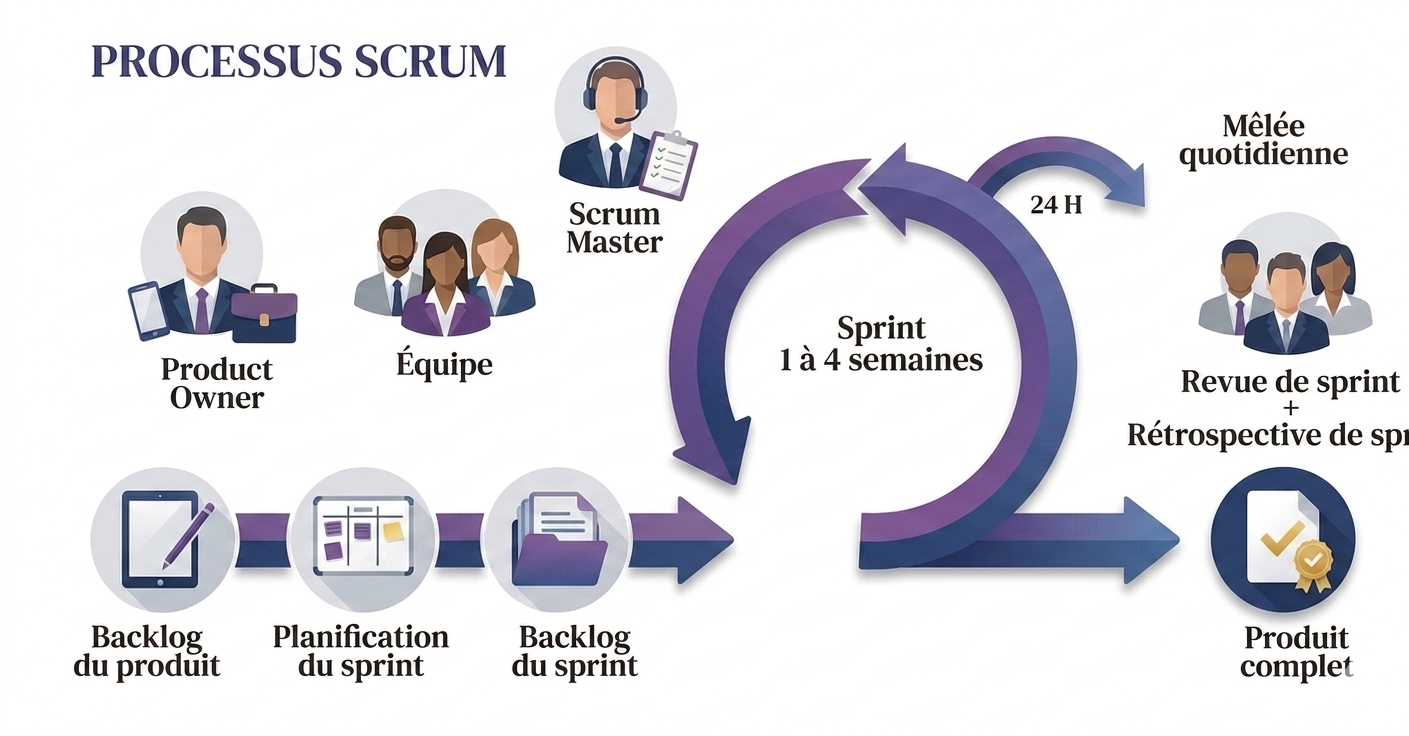
\includegraphics[width=12cm]{images/scrumWhite.png}
}{%
    \fbox{\begin{minipage}{10cm}
    \centering
    \vspace{3cm}
    \textit{Cycle de vie Scrum}
    \vspace{3cm}
    \end{minipage}}
}
\caption{Cycle de vie d'un projet Scrum}
\end{figure}

\subsection{L'équipe SCRUM}

\begin{table}[H]
\centering
\begin{tabular}{|p{4cm}|p{10cm}|}
\hline
\textbf{Rôle} & \textbf{Responsabilités} \\
\hline
Product Owner & Définition des besoins et priorités du projet \\
\hline
Scrum Master & Supervision de la méthodologie SCRUM \\
\hline
Équipe de développement & Développement et implémentation des fonctionnalités \\
\hline
\end{tabular}
\caption{Les rôles SCRUM}
\end{table}

% ==================================================
% CONCLUSION CHAPITRE 1
% ==================================================

\section{Conclusion}

Dans ce chapitre, j'ai présenté le cadre général du projet ainsi que l'organisme d'accueil We Are Tech.

J'ai également étudié les solutions existantes (Properstar, Mubawab et la gestion manuelle) afin d'identifier leurs limites et proposer une solution adaptée aux besoins du domaine immobilier moderne.

Enfin, j'ai présenté la méthodologie SCRUM adoptée ainsi que les outils utilisés pour la gestion et le développement du projet.

Dans le chapitre suivant, je présenterai l'initiation du projet ainsi que l'étude technique de la plateforme.

% ==================================================
% CHAPITRE 2 : INITIATION DU PROJET ET ÉTUDE TECHNIQUE
% ==================================================

\chapter{Initiation du projet et étude technique}

\minitoc

% ==================================================
% INTRODUCTION
% ==================================================

\section{Introduction}

La réussite d'un projet informatique de grande envergure repose avant tout sur une phase d'analyse et de conception rigoureuse, menée en amont de toute activité de développement. Cette étape fondamentale permet de définir avec précision le périmètre fonctionnel du système, d'identifier les acteurs concernés, de recenser les besoins exprimés et de choisir les technologies les mieux adaptées aux objectifs poursuivis.

Dans ce chapitre, nous consacrons notre attention à l'initiation formelle du projet \textbf{Maison3D Immobilier} et à son étude technique approfondie. Nous commençons par présenter les objectifs stratégiques du projet, puis nous identifions et décrivons en détail les différents acteurs du système. Nous enchaînons ensuite avec une analyse complète des besoins fonctionnels et non fonctionnels, avant de présenter l'architecture générale et technique de la plateforme. Nous consacrons une section aux choix technologiques retenus et justifions chaque décision technique. Enfin, nous exposons les différents diagrammes UML réalisés dans le cadre de la modélisation du système.

% ==================================================
% SECTION 2 : OBJECTIFS DU PROJET
% ==================================================

\section{Objectifs du projet}

\subsection{Objectif principal}

L'objectif principal du projet \textbf{Maison3D Immobilier} est de concevoir et développer une plateforme web immobilière moderne, sécurisée et évolutive, permettant aux agences immobilières de centraliser l'ensemble de leurs opérations au sein d'un seul et même outil numérique. La plateforme vise à remplacer les processus manuels et les outils fragmentés par une solution intégrée répondant aux exigences du marché immobilier actuel.

\subsection{Objectifs spécifiques}

Le projet \textbf{Maison3D Immobilier} poursuit plusieurs objectifs spécifiques qui peuvent être organisés selon les axes suivants :

\subsubsection{Axe organisationnel}

\begin{itemize}
    \item Centraliser la gestion des agences immobilières, des biens et des utilisateurs au sein d'une interface unique et cohérente.
    \item Mettre en place une gestion hiérarchique des rôles permettant d'adapter les fonctionnalités selon chaque type d'utilisateur.
    \item Automatiser certaines opérations récurrentes telles que le suivi des contrats, la gestion des renouvellements et le calcul des commissions.
    \item Améliorer la collaboration interne entre les membres des équipes grâce à une messagerie professionnelle intégrée.
\end{itemize}

\subsubsection{Axe commercial}

\begin{itemize}
    \item Faciliter la gestion des transactions immobilières (ventes et locations) avec un suivi complet de chaque opération.
    \item Permettre l'intégration d'un réseau d'affiliés indépendants capables d'apporter des clients potentiels à l'agence en échange de commissions.
    \item Offrir un portail public permettant aux clients de consulter les biens disponibles et d'entrer en contact avec les agences.
    \item Mettre en place un système de commissions transparent et traçable pour les affiliés et les commerciaux.
\end{itemize}

\subsubsection{Axe technique}

\begin{itemize}
    \item Développer une architecture robuste, performante et évolutive basée sur Angular et Spring Boot.
    \item Garantir la sécurité des données grâce à une authentification JWT et une gestion fine des permissions.
    \item Intégrer des fonctionnalités avancées telles que la géolocalisation des biens, la visualisation 3D et les tableaux de bord intelligents.
    \item Assurer la scalabilité de la plateforme pour supporter un nombre croissant d'agences et d'utilisateurs.
\end{itemize}

% ==================================================
% SECTION 3 : IDENTIFICATION DES ACTEURS
% ==================================================

\section{Identification des acteurs du système}

Un acteur représente tout entité externe qui interagit avec le système. Dans le cadre de la plateforme \textbf{Maison3D Immobilier}, six acteurs principaux ont été identifiés, chacun disposant d'un périmètre d'actions bien défini.

\begin{table}[H]
\centering
\begin{tabular}{|p{4.5cm}|p{10cm}|}
\hline
\textbf{Acteur} & \textbf{Description générale} \\
\hline
SUPER\_ADMIN & Administrateur global de la plateforme. Supervise l'ensemble de l'écosystème. \\
\hline
ADMIN & Administrateur d'une agence immobilière. Gère son agence et son équipe. \\
\hline
RESPONSABLE\_COMMERCIAL & Supervise les activités commerciales au sein de l'agence. \\
\hline
COMMERCIAL & Agent immobilier responsable de la gestion opérationnelle des biens. \\
\hline
AFFILIATE & Partenaire externe apportant des clients potentiels contre commissions. \\
\hline
CLIENT\_PUBLIC & Visiteur ou prospect consultant les biens via le portail public. \\
\hline
\end{tabular}
\caption{Identification des acteurs du système Maison3D Immobilier}
\end{table}

% ==================================================
% SECTION 4 : DESCRIPTION DÉTAILLÉE DES ACTEURS
% ==================================================

\section{Description détaillée des acteurs}

\subsection{SUPER\_ADMIN}

Le \textbf{SUPER\_ADMIN} représente l'administrateur global de la plateforme \textbf{Maison3D Immobilier}. Il possède un accès complet à l'ensemble du système et intervient à un niveau transversal, au-dessus de toutes les agences.

Ses principales responsabilités sont les suivantes :

\begin{itemize}
    \item Approuver les demandes d'inscription des nouvelles agences immobilières sur la plateforme.
    \item Consulter et superviser l'ensemble des agences, des utilisateurs et des biens présents sur la plateforme.
    \item Gérer les affiliés globaux et superviser les paiements de zones.
    \item Accéder aux statistiques globales et aux tableaux de bord de synthèse permettant de visualiser les indicateurs de performance de la plateforme.
    \item Communiquer avec les administrateurs des agences via la messagerie interne.
    \item Gérer les demandes de partage de biens entre agences et les valider ou les rejeter.
    \item Superviser les commissions et les transactions au niveau global.
\end{itemize}

\subsection{ADMIN}

L'\textbf{ADMIN} représente l'administrateur d'une agence immobilière. Il est responsable de la gestion complète de son agence et de toute son équipe interne.

Ses principales responsabilités sont les suivantes :

\begin{itemize}
    \item Gérer les utilisateurs de son agence, notamment la création, la modification et la désactivation des comptes des commerciaux et des responsables commerciaux.
    \item Valider ou rejeter les biens immobiliers soumis par les commerciaux de son agence.
    \item Gérer les affiliés rattachés à son agence, approuver leurs profils et superviser leurs activités.
    \item Suivre et gérer les transactions de vente et de location réalisées par son agence.
    \item Gérer les commissions dues aux commerciaux et aux affiliés.
    \item Consulter le tableau de bord de son agence avec les indicateurs clés de performance.
    \item Communiquer avec les membres de son équipe via la messagerie interne.
    \item Accepter ou rejeter les offres soumises par les affiliés concernant les biens de son agence.
\end{itemize}

\subsection{RESPONSABLE\_COMMERCIAL}

Le \textbf{RESPONSABLE\_COMMERCIAL} occupe un rôle intermédiaire entre l'ADMIN et les commerciaux. Il supervise les activités commerciales de l'agence et coordonne l'équipe de vente.

Ses principales responsabilités sont les suivantes :

\begin{itemize}
    \item Gérer les biens immobiliers de l'agence, notamment leur création et leur modification.
    \item Superviser les activités des commerciaux et suivre leurs performances.
    \item Suivre les transactions de vente et de location en cours.
    \item Communiquer avec les membres de l'équipe via la messagerie interne.
    \item Consulter les statistiques commerciales de l'agence via le tableau de bord.
    \item Gérer les statuts des biens immobiliers selon l'avancement des opérations.
\end{itemize}

\subsection{COMMERCIAL}

Le \textbf{COMMERCIAL} est l'agent immobilier opérationnel. Il intervient directement dans la gestion quotidienne des biens et des clients.

Ses principales responsabilités sont les suivantes :

\begin{itemize}
    \item Ajouter, modifier et gérer les biens immobiliers de l'agence, incluant l'upload des images, la géolocalisation et la description détaillée.
    \item Gérer les clients associés aux biens dont il a la charge.
    \item Suivre les transactions de vente et de location qui lui sont attribuées.
    \item Mettre à jour les statuts des biens selon l'avancement des opérations commerciales.
    \item Communiquer avec les membres de l'équipe via la messagerie interne.
    \item Consulter son tableau de bord personnel avec ses indicateurs de performance.
\end{itemize}

\subsection{AFFILIATE}

L'\textbf{AFFILIATE} est un partenaire commercial externe, indépendant de l'agence, qui apporte des clients potentiels intéressés par des biens immobiliers. En contrepartie, il perçoit une commission basée sur le pourcentage défini sur le bien vendu ou loué.

Ses principales caractéristiques sont les suivantes :

\begin{itemize}
    \item Il s'inscrit de manière autonome sur la plateforme et attend l'approbation de son profil.
    \item Il sélectionne des zones géographiques (pays, ville) dans lesquelles il souhaite opérer. La première zone est gratuite ; les zones supplémentaires nécessitent un paiement.
    \item Il consulte les biens disponibles dans ses zones d'intervention et soumet des offres de vente au nom de ses clients.
    \item Il suit l'évolution de ses offres (en attente, acceptée, rejetée, complétée) via son espace personnel.
    \item Il consulte ses commissions générées et son classement parmi les affiliés de la plateforme.
    \item Il communique avec les agences via la messagerie interne.
\end{itemize}

\subsection{CLIENT\_PUBLIC}

Le \textbf{CLIENT\_PUBLIC} représente tout visiteur ou prospect qui accède à la plateforme via le portail public. Il peut créer un compte et interagir avec les agences.

Ses interactions avec la plateforme sont les suivantes :

\begin{itemize}
    \item Consulter les biens immobiliers disponibles sur le portail public.
    \item Rechercher et filtrer les biens selon des critères spécifiques (prix, localisation, superficie, catégorie).
    \item Consulter les détails complets d'un bien, y compris les photos, la géolocalisation et la description.
    \item Manifester son intérêt pour un bien, ce qui génère automatiquement un lead dans le CRM de l'agence concernée.
    \item Contacter directement une agence via la messagerie intégrée.
    \item Bénéficier d'une expérience de visualisation 3D pour les biens premium dotés de modèles 3D.
\end{itemize}

% ==================================================
% SECTION 5 : BESOINS FONCTIONNELS
% ==================================================

\section{Besoins fonctionnels}

Les besoins fonctionnels décrivent l'ensemble des fonctionnalités que le système doit offrir pour répondre aux attentes des utilisateurs identifiés. Ils sont organisés par modules afin de faciliter leur lecture et leur compréhension.

\subsection{Module Authentification et Sécurité}

Le module d'authentification constitue le point d'entrée de la plateforme. Il doit assurer un accès sécurisé et contrôlé à tous les utilisateurs.

\begin{itemize}
    \item \textbf{Connexion sécurisée :} L'utilisateur doit pouvoir se connecter à la plateforme en saisissant son adresse email et son mot de passe. Les credentials sont vérifiés côté serveur et un token JWT est généré en cas de succès.
    \item \textbf{Gestion du profil :} Chaque utilisateur doit pouvoir consulter et modifier ses informations personnelles (nom, prénom, téléphone, photo de profil).
    \item \textbf{Modification du mot de passe :} L'utilisateur doit pouvoir modifier son mot de passe après vérification de l'ancien.
    \item \textbf{Déconnexion sécurisée :} La déconnexion invalide le token JWT côté client.
    \item \textbf{Gestion des rôles :} Le système doit adapter dynamiquement les fonctionnalités et l'interface utilisateur selon le rôle de l'utilisateur connecté.
    \item \textbf{Protection des APIs :} Chaque endpoint REST doit être protégé par une vérification du token JWT et du rôle requis.
    \item \textbf{Création des comptes :} Le SUPER\_ADMIN et l'ADMIN peuvent créer des comptes pour les utilisateurs de leur périmètre.
    \item \textbf{Activation / désactivation :} Les comptes peuvent être activés ou désactivés sans suppression des données historiques.
\end{itemize}

\subsection{Module Gestion des Agences}

\begin{itemize}
    \item \textbf{Inscription d'une agence :} Une agence peut s'inscrire de manière autonome sur la plateforme. La demande d'inscription est soumise à l'approbation du SUPER\_ADMIN.
    \item \textbf{Approbation / rejet :} Le SUPER\_ADMIN peut approuver ou rejeter les demandes d'inscription des agences.
    \item \textbf{Gestion des informations :} L'ADMIN peut modifier les informations de son agence (nom, adresse, logo, contact).
    \item \textbf{Consultation globale :} Le SUPER\_ADMIN peut consulter la liste complète de toutes les agences présentes sur la plateforme avec leurs statistiques.
    \item \textbf{Partage de biens entre agences :} Le système doit permettre à une agence de proposer le partage d'un bien avec une autre agence, avec un workflow d'approbation dédié.
\end{itemize}

\subsection{Module Gestion des Biens Immobiliers}

Ce module constitue le cœur fonctionnel de la plateforme. Il gère l'ensemble du cycle de vie des biens immobiliers.

\begin{itemize}
    \item \textbf{Ajout d'un bien :} Le commercial peut créer une fiche détaillée pour un bien immobilier en renseignant le titre, la description, le prix, la superficie, le nombre de pièces, le type, la catégorie et l'adresse complète.
    \item \textbf{Upload d'images :} Le système doit permettre l'upload de plusieurs images pour chaque bien. Une image principale est désignée pour la vignette d'aperçu.
    \item \textbf{Géolocalisation :} Le bien doit être géolocalisé automatiquement via l'API Leaflet Maps à partir de l'adresse saisie. L'utilisateur peut également ajuster manuellement la position sur la carte.
    \item \textbf{Validation par l'Admin :} Tout bien nouvellement créé est soumis à la validation de l'ADMIN avant d'être visible sur le portail public.
    \item \textbf{Gestion des statuts :} Le système doit gérer quatre statuts distincts pour les biens immobiliers, selon la logique décrite dans le tableau~\ref{tab:statuts-biens} (voir ci-dessous).
    \item \textbf{Modification et suppression :} Le commercial peut modifier les informations d'un bien tant qu'il n'est pas dans un statut verrouillé.
    \item \textbf{Historique des modifications :} Le système conserve l'historique de toutes les modifications apportées à chaque bien.
    \item \textbf{Définition de la commission affilié :} L'ADMIN peut définir un pourcentage de commission sur chaque bien, utilisé pour le calcul des commissions des affiliés.
\end{itemize}

\begin{table}[H]
\centering
\begin{tabular}{|p{3cm}|p{5cm}|p{6cm}|}
\hline
\textbf{Statut} & \textbf{Description} & \textbf{Comportement système} \\
\hline
DISPONIBLE & Bien disponible à la vente ou à la location & Visible sur le portail public, modifiable \\
\hline
EN\_ATTENTE & Bien soumis en attente de validation & Non visible publiquement, en attente Admin \\
\hline
VENDU & Bien définitivement vendu & Statut verrouillé, transaction de vente générée automatiquement, bien retiré des listings \\
\hline
LOUÉ & Bien en location active & Statut verrouillé pendant la durée du contrat, transaction de location générée, déverrouillage automatique à l'expiration \\
\hline
\end{tabular}
\caption{Logique des statuts des biens immobiliers}
\label{tab:statuts-biens}
\end{table}

\subsection{Module Gestion des Transactions}

\begin{itemize}
    \item \textbf{Transactions de vente :} Toute vente d'un bien génère automatiquement une transaction de vente enregistrant la date, le montant, les parties impliquées et les notes associées.
    \item \textbf{Transactions de location :} Toute mise en location génère une transaction avec les dates de début et de fin, le montant du loyer et le contrat associé.
    \item \textbf{Gestion des contrats :} Le système gère les contrats de location en suivant leur durée et en déclenchant des alertes avant leur expiration.
    \item \textbf{Renouvellements :} Le système identifie automatiquement les contrats arrivant à échéance et permet leur renouvellement simplifié.
    \item \textbf{Contrats expirés :} Les contrats expirés sont archivés et les biens correspondants reprennent le statut DISPONIBLE automatiquement.
    \item \textbf{Historique des transactions :} Chaque acteur dispose d'un accès à l'historique complet des transactions selon son périmètre de visibilité.
\end{itemize}

\subsection{Module Messagerie Interne}

\begin{itemize}
    \item \textbf{Messagerie temps réel :} Les utilisateurs peuvent échanger des messages en temps réel au sein de la plateforme.
    \item \textbf{Conversations :} Le système organise les échanges sous forme de conversations entre deux utilisateurs ou groupes d'utilisateurs.
    \item \textbf{Notifications de nouveaux messages :} Lorsqu'un nouveau message est reçu, l'utilisateur en est notifié via une icône dans l'interface.
    \item \textbf{Messages non lus :} Le système affiche un compteur de messages non lus et permet de les marquer comme lus.
    \item \textbf{Historique des messages :} L'historique complet de chaque conversation est conservé et accessible à tout moment.
    \item \textbf{Aperçu du dernier message :} La liste des conversations affiche un aperçu du dernier message échangé et son horodatage.
    \item \textbf{Recherche d'utilisateurs :} L'utilisateur peut rechercher d'autres utilisateurs pour initier une nouvelle conversation.
\end{itemize}

\subsection{Module Gestion des Affiliés}

\begin{itemize}
    \item \textbf{Inscription des affiliés :} Les affiliés peuvent s'inscrire de manière autonome sur la plateforme. Leur profil est soumis à l'approbation de l'ADMIN ou du SUPER\_ADMIN.
    \item \textbf{Gestion des zones :} Chaque affilié sélectionne les zones géographiques (pays, ville) dans lesquelles il souhaite opérer. La première zone est offerte gratuitement ; les zones premium nécessitent un paiement avec preuve justificative.
    \item \textbf{Catalogue des biens éligibles :} L'affilié dispose d'un catalogue personnalisé regroupant uniquement les biens disponibles dans ses zones d'intervention.
    \item \textbf{Soumission d'offres :} L'affilié peut soumettre des offres de vente ou de location pour les biens de son catalogue, au nom de ses clients potentiels.
    \item \textbf{Suivi des offres :} L'affilié suit l'état de ses offres (EN\_ATTENTE, ACCEPTÉE, REJETÉE, COMPLÉTÉE) en temps réel.
    \item \textbf{Gestion des commissions :} Les commissions sont calculées automatiquement selon le pourcentage défini sur chaque bien lors de la complétion d'une offre.
    \item \textbf{Statistiques affilié :} L'affilié dispose d'un tableau de bord personnel présentant ses performances, ses commissions cumulées et son classement.
    \item \textbf{Classement des affiliés :} Un système de classement permet de distinguer les affiliés les plus performants.
\end{itemize}

\subsection{Module Dashboard Intelligent}

\begin{itemize}
    \item \textbf{Dashboard personnalisé :} Chaque utilisateur dispose d'un tableau de bord adapté à son rôle, présentant les informations les plus pertinentes pour ses activités.
    \item \textbf{Statistiques clés (KPIs) :} Le dashboard présente les indicateurs clés de performance tels que le nombre de biens, le chiffre d'affaires, les transactions récentes et les commissions générées.
    \item \textbf{Activités récentes :} Une liste des dernières actions effectuées sur la plateforme est affichée pour permettre un suivi rapide de l'activité.
    \item \textbf{Notifications :} Les notifications non lues sont mises en évidence sur le dashboard.
    \item \textbf{Validations rapides :} L'ADMIN peut effectuer des validations rapides (biens, affiliés) directement depuis son tableau de bord.
    \item \textbf{Graphiques et visualisations :} Des graphiques interactifs (barres, courbes, camemberts) permettent de visualiser les données statistiques.
\end{itemize}

% ==================================================
% SECTION 6 : BESOINS NON FONCTIONNELS
% ==================================================

\section{Besoins non fonctionnels}

Les besoins non fonctionnels définissent les contraintes et les critères de qualité que le système doit respecter indépendamment des fonctionnalités métier. Ils sont aussi importants que les besoins fonctionnels car ils déterminent la qualité globale de la solution.

\subsection{Sécurité}

La sécurité est une exigence critique pour une plateforme de gestion immobilière manipulant des données sensibles (transactions financières, informations personnelles, contrats).

\begin{itemize}
    \item \textbf{Authentification JWT :} Toutes les requêtes vers les APIs sécurisées doivent être accompagnées d'un token JWT valide signé avec l'algorithme HS256.
    \item \textbf{Hachage des mots de passe :} Les mots de passe sont systématiquement hachés avec l'algorithme BCrypt avant stockage en base de données.
    \item \textbf{Protection des APIs :} Chaque endpoint REST est protégé par des règles d'autorisation basées sur les rôles, configurées via Spring Security.
    \item \textbf{Isolation multi-tenant :} Les données d'une agence ne sont en aucun cas accessibles par les utilisateurs d'une autre agence.
    \item \textbf{Images sécurisées :} Les images sensibles (preuves de paiement) ne sont accessibles que via des requêtes HTTP authentifiées avec le token JWT.
    \item \textbf{Validation des données :} Les données saisies par l'utilisateur sont validées côté frontend (formulaires réactifs Angular) et côté backend (annotations de validation Spring).
    \item \textbf{Configuration CORS :} Une seule source CORS autorisée est définie dans la configuration Spring Security afin d'éviter les attaques cross-origin.
\end{itemize}

\subsection{Performance}

\begin{itemize}
    \item \textbf{Rapidité des réponses :} Les requêtes courantes (consultation de listes, chargement de tableaux de bord) doivent retourner une réponse en moins de deux secondes.
    \item \textbf{Optimisation des requêtes JPA :} Les requêtes en base de données doivent être optimisées pour éviter les problèmes N+1 grâce à l'utilisation de \texttt{@EntityGraph} et de requêtes JPQL adaptées.
    \item \textbf{Architecture Single Page Application :} L'utilisation d'Angular en mode SPA garantit une expérience utilisateur fluide sans rechargement complet de la page.
    \item \textbf{Pagination :} Les listes volumineuses (biens, transactions, utilisateurs) sont paginées côté serveur afin de limiter la quantité de données transférées.
\end{itemize}

\subsection{Disponibilité et Fiabilité}

\begin{itemize}
    \item \textbf{Containerisation Docker :} L'application est conteneurisée avec Docker pour garantir la reproductibilité des déploiements et faciliter la montée en charge.
    \item \textbf{Gestion des erreurs :} Un gestionnaire global d'exceptions (\texttt{GlobalExceptionHandler}) intercepte les erreurs applicatives et retourne des réponses d'erreur standardisées.
    \item \textbf{Logs applicatifs :} Les événements importants (connexions, erreurs, transactions) sont consignés dans des journaux applicatifs pour faciliter le diagnostic.
\end{itemize}

\subsection{Ergonomie et Accessibilité}

\begin{itemize}
    \item \textbf{Interface responsive :} L'interface utilisateur est développée avec Bootstrap 5 pour s'adapter à toutes les tailles d'écran (ordinateur, tablette, mobile).
    \item \textbf{Expérience utilisateur cohérente :} La navigation dans l'application doit être intuitive, avec des retours visuels clairs pour chaque action (loaders, messages de succès ou d'erreur).
    \item \textbf{Internationalisation :} L'interface est développée en français avec une architecture permettant l'ajout futur d'autres langues.
    \item \textbf{Accessibilité WCAG :} Les composants de l'interface respectent les bonnes pratiques d'accessibilité pour les utilisateurs en situation de handicap.
\end{itemize}

\subsection{Maintenabilité et Évolutivité}

\begin{itemize}
    \item \textbf{Architecture modulaire :} Le frontend Angular est organisé en modules indépendants (AuthModule, DashboardModule, PropertyModule, etc.) pour faciliter la maintenabilité.
    \item \textbf{Séparation des responsabilités :} L'architecture backend respecte le principe de séparation des couches (Controller, Service, Repository).
    \item \textbf{Documentation API :} L'API REST est documentée via Swagger UI accessible à l'URL \texttt{/swagger-ui.html}.
    \item \textbf{Versioning Git :} Le code source est versionné sur GitHub avec des branches dédiées par fonctionnalité.
    \item \textbf{Tests unitaires :} Des tests unitaires sont mis en place côté frontend (Vitest) et côté backend (JUnit) pour garantir la non-régression.
\end{itemize}

\begin{table}[H]
\centering
\begin{tabular}{|p{4cm}|p{5cm}|p{5cm}|}
\hline
\textbf{Critère} & \textbf{Exigence} & \textbf{Moyen de satisfaction} \\
\hline
Sécurité & Authentification forte, isolation des données & JWT, BCrypt, Spring Security \\
\hline
Performance & Temps de réponse $<$ 2s & Pagination, optimisation JPA \\
\hline
Disponibilité & Déploiement reproductible & Docker \\
\hline
Ergonomie & Interface responsive & Bootstrap 5, Angular \\
\hline
Maintenabilité & Code modulaire documenté & Architecture en couches, Swagger \\
\hline
Évolutivité & Ajout facile de fonctionnalités & Modules Angular, Services Spring \\
\hline
\end{tabular}
\caption{Récapitulatif des besoins non fonctionnels}
\end{table}

% ==================================================
% SECTION 7 : ARCHITECTURE GÉNÉRALE
% ==================================================

\section{Architecture générale du système}

\subsection{Vue d'ensemble}

La plateforme \textbf{Maison3D Immobilier} repose sur une architecture client-serveur en trois couches, communément appelée architecture \textit{3-Tiers}. Cette architecture organise le système en trois niveaux distincts et indépendants, chacun ayant une responsabilité bien définie.

\begin{itemize}
    \item \textbf{Couche présentation (Frontend) :} Développée avec Angular 21, cette couche constitue l'interface utilisateur de l'application. Elle est exécutée directement dans le navigateur du client sous forme d'une Single Page Application (SPA). Elle est responsable de l'affichage des données, de la validation des formulaires et de l'interaction avec l'utilisateur.
    \item \textbf{Couche métier (Backend) :} Développée avec Spring Boot 3.2, cette couche expose une API REST sécurisée consommée par le frontend. Elle est responsable de l'implémentation de toute la logique métier, du traitement des requêtes, de l'application des règles de gestion et de la gestion de la sécurité.
    \item \textbf{Couche données (Base de données) :} Assurée par MySQL 8.0, cette couche garantit le stockage persistant, fiable et structuré de l'ensemble des données de l'application.
\end{itemize}

\subsection{Flux de communication}

La communication entre les couches s'effectue selon le schéma suivant :

\begin{itemize}
    \item Le frontend Angular communique avec le backend via des requêtes HTTP/HTTPS vers les endpoints REST de l'API Spring Boot. Chaque requête (à l'exception des endpoints publics) inclut un token JWT dans l'en-tête \texttt{Authorization}.
    \item Le backend Spring Boot traite les requêtes reçues, applique les règles de gestion et interagit avec la base de données MySQL via Spring Data JPA / Hibernate.
    \item Les réponses sont retournées au frontend sous forme de payloads JSON.
    \item Les assets statiques (images des biens, preuves de paiement) sont stockés sur le serveur et accessibles via des URLs dédiées, protégées ou publiques selon leur nature.
\end{itemize}

% ==================================================
% SECTION 8 : ARCHITECTURE TECHNIQUE
% ==================================================

\section{Architecture technique détaillée}

\subsection{Architecture Backend}

Le backend est développé avec \textbf{Spring Boot 3.2} et suit une architecture en couches strictement respectée :

\begin{itemize}
    \item \textbf{Couche Controller :} Regroupe les contrôleurs REST responsables de la réception des requêtes HTTP et du retour des réponses. Chaque module fonctionnel dispose de son propre contrôleur (\texttt{AuthController}, \texttt{PropertyController}, \texttt{AffiliateController}, \texttt{DashboardController}, etc.).
    \item \textbf{Couche Service :} Contient la logique métier de l'application. Les services implémentent les règles de gestion, orchestrent les traitements et coordonnent les interactions entre les différents repositories.
    \item \textbf{Couche Repository :} Assure l'accès aux données via Spring Data JPA. Chaque entité dispose de son propre repository avec des requêtes JPQL personnalisées si nécessaire.
    \item \textbf{Couche Entity :} Regroupe les classes JPA mappées sur les tables de la base de données MySQL.
    \item \textbf{Couche DTO :} Contient les objets de transfert de données (Data Transfer Objects) utilisés pour structurer les échanges entre le frontend et le backend.
    \item \textbf{Couche Security :} Regroupe les composants de sécurité : filtre JWT (\texttt{JwtFilter}), service de chargement des utilisateurs (\texttt{UserDetailsService}) et configuration Spring Security (\texttt{SecurityConfig}).
\end{itemize}

\subsection{Architecture Frontend}

Le frontend est développé avec \textbf{Angular 21} en architecture standalone. Il est organisé selon une structure par fonctionnalités :

\begin{itemize}
    \item \textbf{Module Admin :} Regroupe tous les composants de l'interface d'administration (shell, sidebar, header, dashboard, gestion des biens, des transactions, des affiliés, etc.).
    \item \textbf{Module Portail Public :} Regroupe les composants accessibles sans authentification (consultation des biens, formulaire de contact, visualisation 3D).
    \item \textbf{Module Authentification :} Gère les formulaires de connexion, d'inscription et de réinitialisation du mot de passe.
    \item \textbf{Services :} Regroupe les services Angular responsables des appels HTTP vers l'API backend (\texttt{AuthService}, \texttt{PropertyService}, \texttt{AffiliateService}, etc.).
    \item \textbf{Guards :} Les \texttt{AuthGuard} et \texttt{RoleGuard} protègent les routes selon le statut d'authentification et le rôle de l'utilisateur.
    \item \textbf{Intercepteurs HTTP :} Le \texttt{JwtInterceptor} injecte automatiquement le token JWT dans les en-têtes de toutes les requêtes HTTP sortantes.
\end{itemize}

% ==================================================
% SECTION 9 : CHOIX TECHNOLOGIQUES
% ==================================================

\section{Choix technologiques}

\subsection{Frontend : Angular 21}

Angular a été choisi comme framework frontend pour les raisons suivantes :

\begin{itemize}
    \item \textbf{Architecture TypeScript :} Angular impose l'utilisation de TypeScript, ce qui améliore la robustesse du code grâce au typage statique et à la détection précoce des erreurs.
    \item \textbf{Architecture modulaire :} La structure en modules standalone d'Angular 21 facilite la séparation des responsabilités et l'organisation du code.
    \item \textbf{Formulaires réactifs :} Les Reactive Forms d'Angular offrent une gestion puissante et flexible des formulaires complexes avec validation intégrée.
    \item \textbf{Injection de dépendances :} Le système d'injection de dépendances natif d'Angular facilite la gestion des services et améliore la testabilité du code.
    \item \textbf{Routing avancé :} Le routeur Angular supporte les guards, les resolvers et la navigation programmatique, indispensables pour une application multi-rôles.
    \item \textbf{Intégration RxJS :} La programmation réactive avec RxJS permet une gestion efficace des flux de données asynchrones.
\end{itemize}

\begin{table}[H]
\centering
\begin{tabular}{|p{4cm}|p{10cm}|}
\hline
\textbf{Bibliothèque} & \textbf{Utilisation dans le projet} \\
\hline
Bootstrap 5 & Framework CSS pour le design responsive de l'interface \\
\hline
Leaflet + Leaflet Draw & Cartographie interactive et géolocalisation des biens \\
\hline
Three.js & Visualisation 3D des biens immobiliers premium \\
\hline
ApexCharts & Graphiques et visualisations des statistiques du dashboard \\
\hline
RxJS & Gestion des flux de données asynchrones \\
\hline
\end{tabular}
\caption{Bibliothèques frontend utilisées dans le projet}
\end{table}

\subsection{Backend : Spring Boot 3.2}

Spring Boot 3.2 avec Java 17 a été choisi pour les raisons suivantes :

\begin{itemize}
    \item \textbf{Productivité :} Spring Boot offre une configuration automatique et une mise en route rapide grâce à ses starters, réduisant considérablement le temps de configuration.
    \item \textbf{Écosystème Spring :} L'écosystème Spring (Spring Security, Spring Data JPA, Spring MVC) fournit des solutions éprouvées pour les besoins les plus courants d'une application d'entreprise.
    \item \textbf{Sécurité robuste :} Spring Security, combiné à JJWT pour la gestion des tokens JWT, offre une sécurisation complète et flexible des APIs REST.
    \item \textbf{Spring Data JPA :} Simplifie considérablement l'accès aux données grâce à la génération automatique des requêtes et aux repositories.
    \item \textbf{Java 17 :} La dernière version LTS de Java apporte des améliorations de performance et de nouvelles fonctionnalités du langage (records, sealed classes, pattern matching).
    \item \textbf{Documentation Swagger :} L'intégration de Swagger UI via SpringDoc OpenAPI permet de documenter automatiquement l'ensemble des endpoints REST.
\end{itemize}

\subsection{Base de données : MySQL 8.0}

MySQL 8.0 a été retenu comme système de gestion de base de données relationnelle pour les raisons suivantes :

\begin{itemize}
    \item \textbf{Maturité et fiabilité :} MySQL est l'un des SGBDR les plus utilisés dans le monde, avec une communauté importante et une documentation exhaustive.
    \item \textbf{Performances :} MySQL 8.0 offre d'excellentes performances pour les opérations de lecture intensive, typiques des applications immobilières.
    \item \textbf{Intégrité référentielle :} Le support complet des contraintes de clés étrangères garantit la cohérence des données.
    \item \textbf{Compatibilité JPA/Hibernate :} MySQL s'intègre parfaitement avec Spring Data JPA et Hibernate, le schéma étant généré automatiquement au démarrage (\texttt{ddl-auto: update}).
    \item \textbf{Coût :} MySQL est disponible en version gratuite (Community Edition), ce qui en fait un choix économiquement pertinent pour un projet universitaire.
\end{itemize}

\subsection{Authentification : JSON Web Token (JWT)}

\begin{itemize}
    \item \textbf{Stateless :} L'authentification JWT est sans état côté serveur, ce qui simplifie l'architecture et facilite la scalabilité horizontale.
    \item \textbf{Portabilité :} Le token JWT est auto-descriptif (il contient le rôle et l'identifiant de l'utilisateur dans son payload), ce qui permet au frontend de prendre des décisions de navigation sans solliciter le serveur.
    \item \textbf{Sécurité :} Le token est signé avec une clé secrète (algorithme HS256), ce qui garantit son intégrité.
    \item \textbf{Expiration :} Chaque token est associé à une durée de validité configurable (24 heures par défaut).
\end{itemize}

\subsection{Infrastructure : Docker et GitHub}

\begin{itemize}
    \item \textbf{Docker :} La containerisation de l'application via Docker garantit la reproductibilité des environnements de développement, de test et de production.
    \item \textbf{GitHub :} Le versioning du code source sur GitHub avec un workflow de branches par fonctionnalité assure la traçabilité des modifications et facilite la collaboration.
\end{itemize}

\begin{table}[H]
\centering
\begin{tabular}{|p{3.5cm}|p{3.5cm}|p{7cm}|}
\hline
\textbf{Composant} & \textbf{Technologie} & \textbf{Justification} \\
\hline
Frontend & Angular 21 & Framework SPA robuste, TypeScript, modules standalone \\
\hline
Backend & Spring Boot 3.2 & Écosystème Spring complet, productivité, sécurité intégrée \\
\hline
Base de données & MySQL 8.0 & SGBDR mature, performant, compatible JPA \\
\hline
Authentification & JWT (JJWT 0.11.5) & Stateless, sécurisé, portabilité du token \\
\hline
Cartographie & Leaflet.js & Open source, léger, riche en plugins \\
\hline
Visualisation 3D & Three.js & Standard web 3D, rendu in-page via \texttt{<model-viewer>} \\
\hline
Graphiques & ApexCharts & Bibliothèque moderne, graphiques interactifs \\
\hline
Infrastructure & Docker + GitHub & Containerisation + versioning \\
\hline
\end{tabular}
\caption{Récapitulatif des choix technologiques}
\end{table}

% ==================================================
% SECTION 10 : DIAGRAMMES UML
% ==================================================

\section{Modélisation UML du système}

La modélisation UML (Unified Modeling Language) constitue une étape fondamentale dans la conception d'un système logiciel. Elle permet de visualiser, spécifier et documenter les aspects structurels et comportementaux du système. Dans le cadre du projet \textbf{Maison3D Immobilier}, plusieurs types de diagrammes UML ont été élaborés afin de couvrir l'ensemble des dimensions du système.

% ==================================================
% 10.1 DIAGRAMME DE CAS D'UTILISATION GLOBAL
% ==================================================

\subsection{Diagramme de cas d'utilisation global}

Le diagramme de cas d'utilisation global offre une vue d'ensemble des interactions entre les acteurs du système et les fonctionnalités principales de la plateforme \textbf{Maison3D Immobilier}. Il met en évidence les six acteurs identifiés et leurs périmètres d'interaction respectifs avec les différents modules du système.

\begin{figure}[H]
\centering
\IfFileExists{images/usecase-global.png}{%
    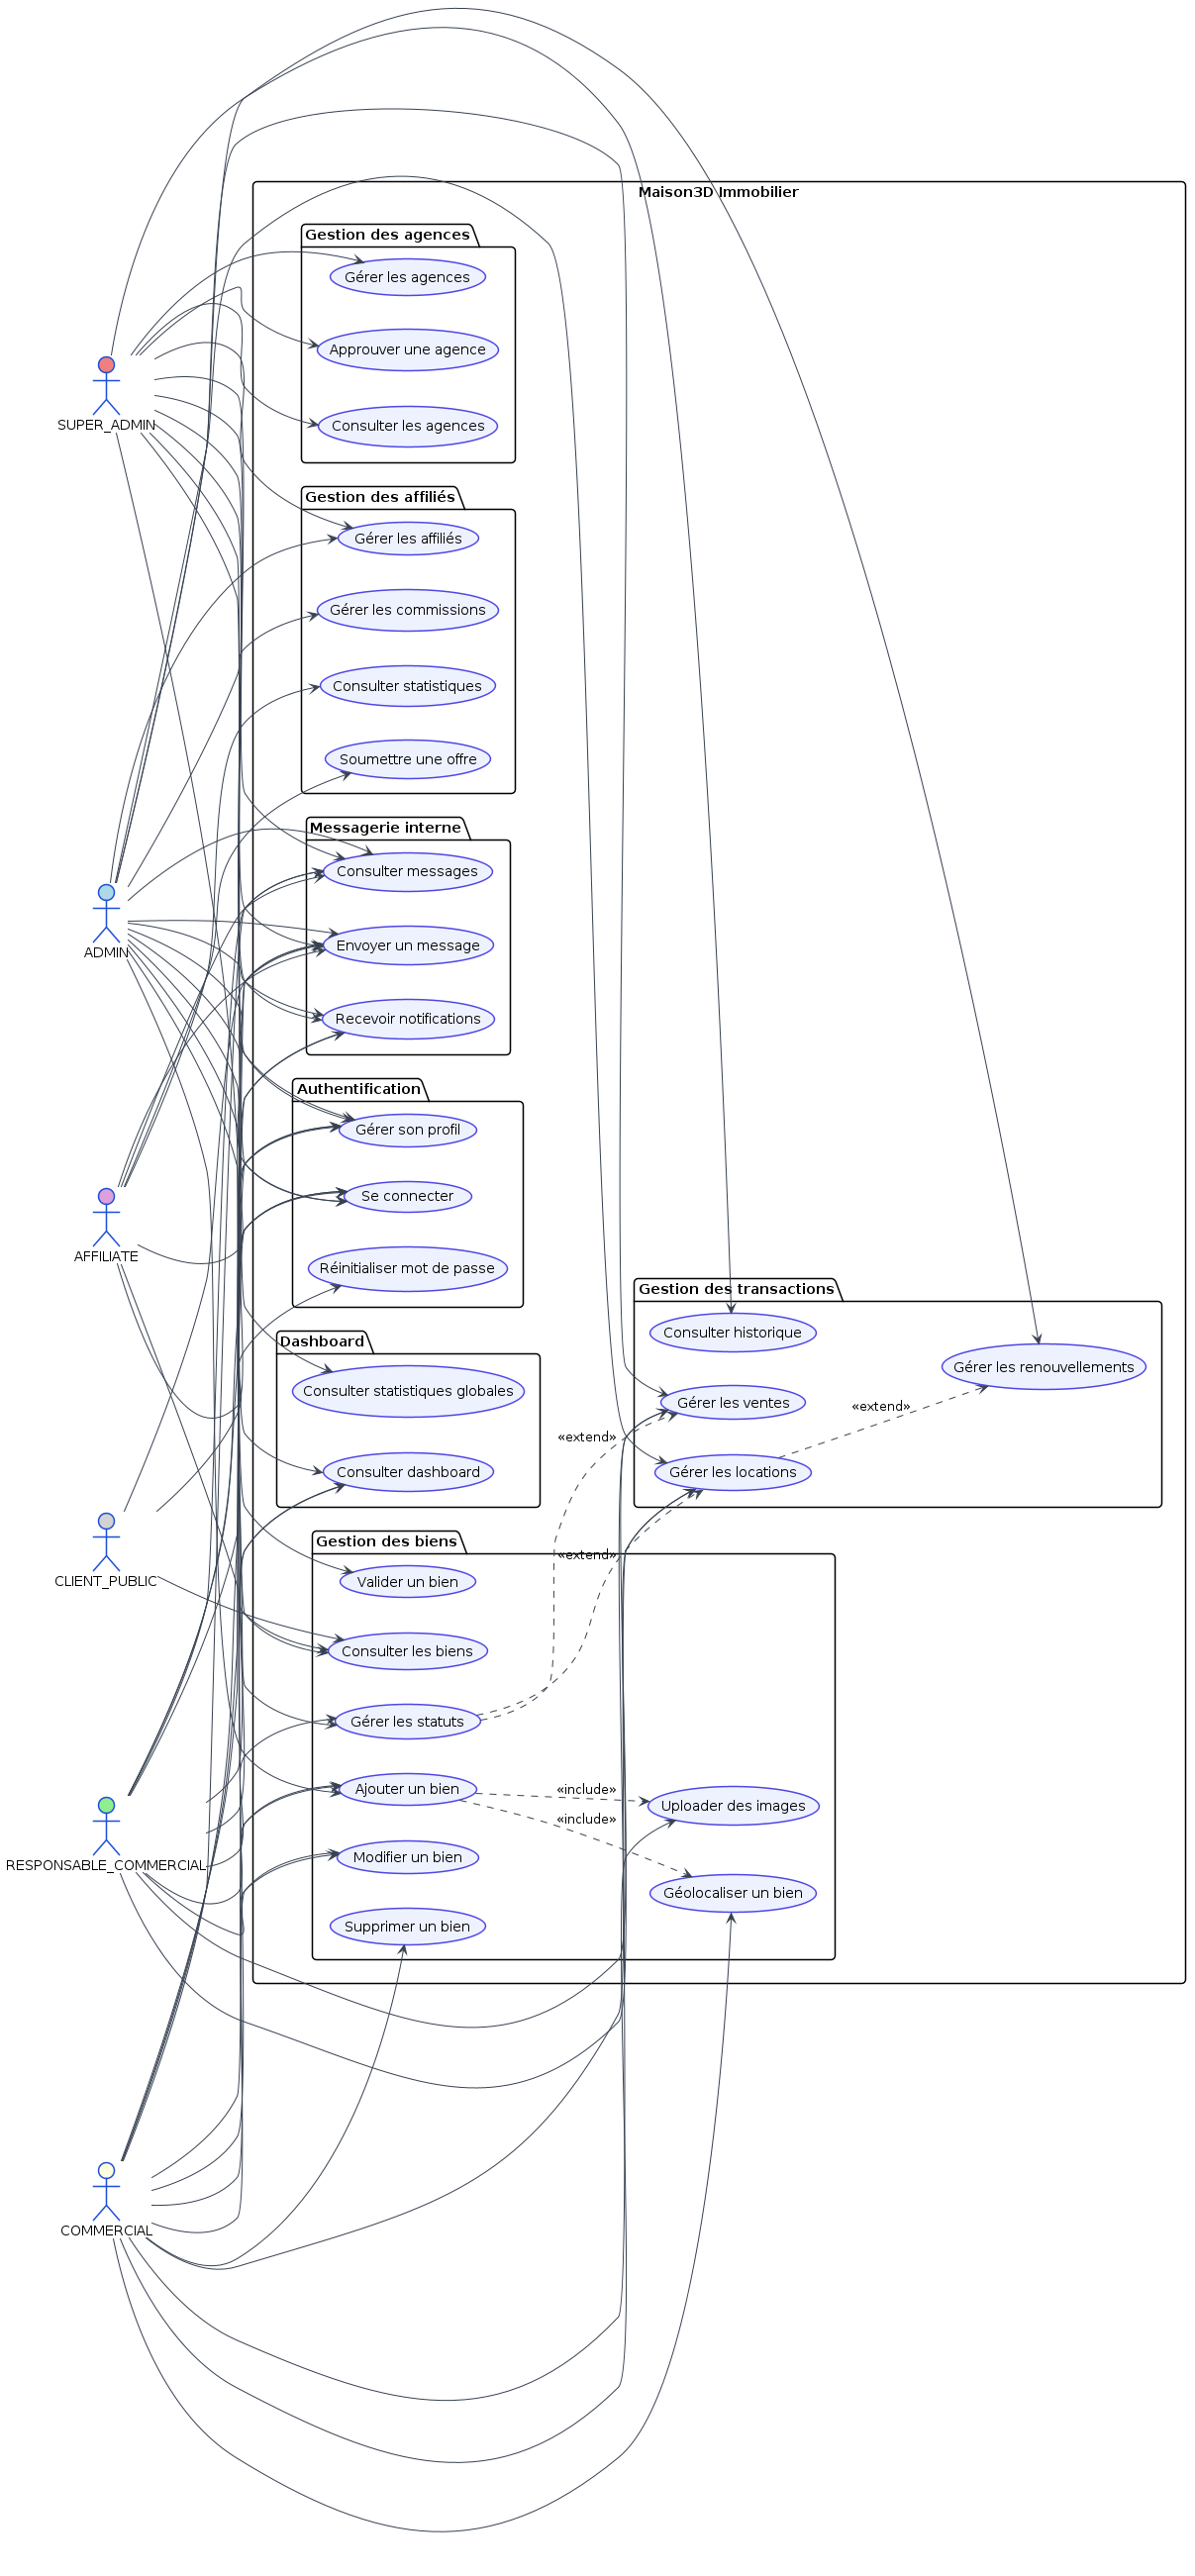
\includegraphics[width=0.95\textwidth]{images/usecase-global.png}
}{%
    \fbox{\begin{minipage}{0.9\textwidth}
    \centering
    \vspace{4cm}
    \textit{[Diagramme de cas d'utilisation global]}
    \vspace{4cm}
    \end{minipage}}
}
\caption{Diagramme de cas d'utilisation global de la plateforme Maison3D Immobilier}
\end{figure}

% ==================================================
% 10.2 DIAGRAMME UC - AUTHENTIFICATION
% ==================================================

\subsection{Diagramme de cas d'utilisation — Module Authentification}

Ce diagramme détaille les cas d'utilisation relatifs au module d'authentification et de sécurité. Il illustre la relation d'héritage entre les acteurs (tous les acteurs héritent de l'acteur générique \textit{Utilisateur}) ainsi que les relations \textit{include} et \textit{extend} entre les cas d'utilisation.

\begin{figure}[H]
\centering
\IfFileExists{images/usecase-auth.png}{%
    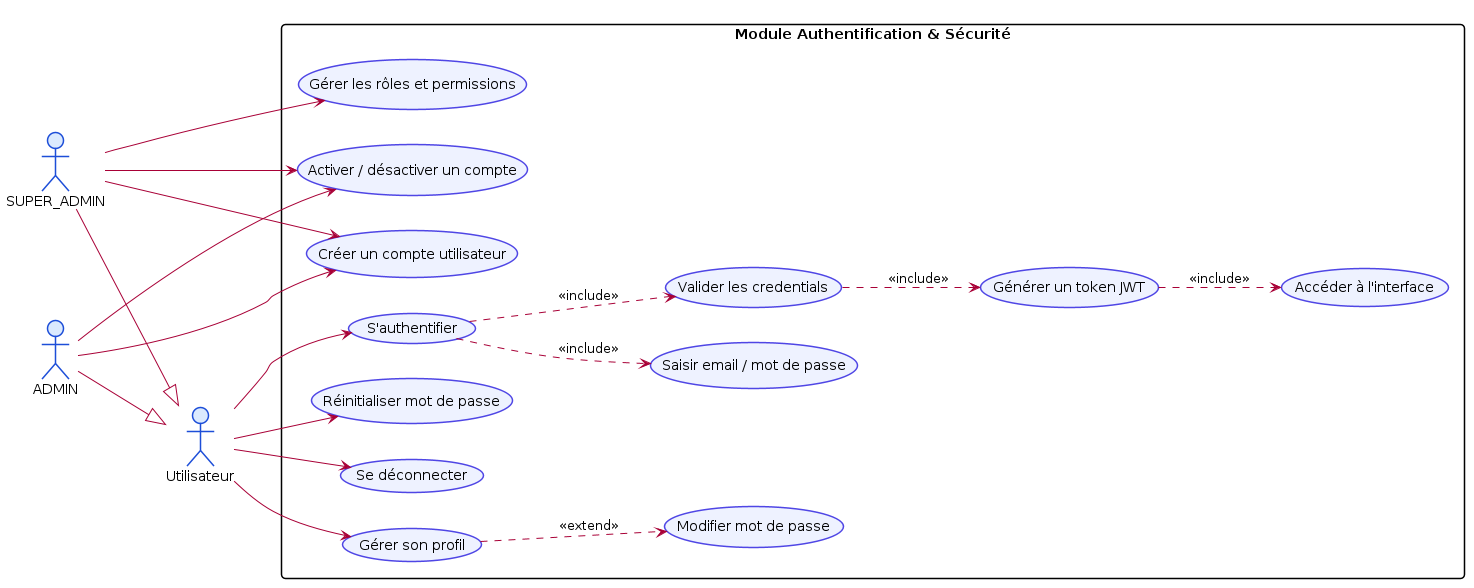
\includegraphics[width=0.85\textwidth]{images/usecase-auth.png}
}{%
    \fbox{\begin{minipage}{0.9\textwidth}
    \centering
    \vspace{4cm}
    \textit{[Diagramme de cas d'utilisation — Authentification]}
    \vspace{4cm}
    \end{minipage}}
}
\caption{Diagramme de cas d'utilisation du module Authentification et Sécurité}
\end{figure}

% ==================================================
% 10.3 DIAGRAMME UC - GESTION DES BIENS
% ==================================================

\subsection{Diagramme de cas d'utilisation — Module Gestion des Biens}

Ce diagramme présente les cas d'utilisation relatifs à la gestion des biens immobiliers. Il illustre les différentes interactions selon les rôles et met en évidence les relations d'inclusion et d'extension entre les cas d'utilisation (l'ajout d'un bien inclut obligatoirement l'upload d'images et la géolocalisation).

\begin{figure}[H]
\centering
\IfFileExists{images/usecase-biens.png}{%
    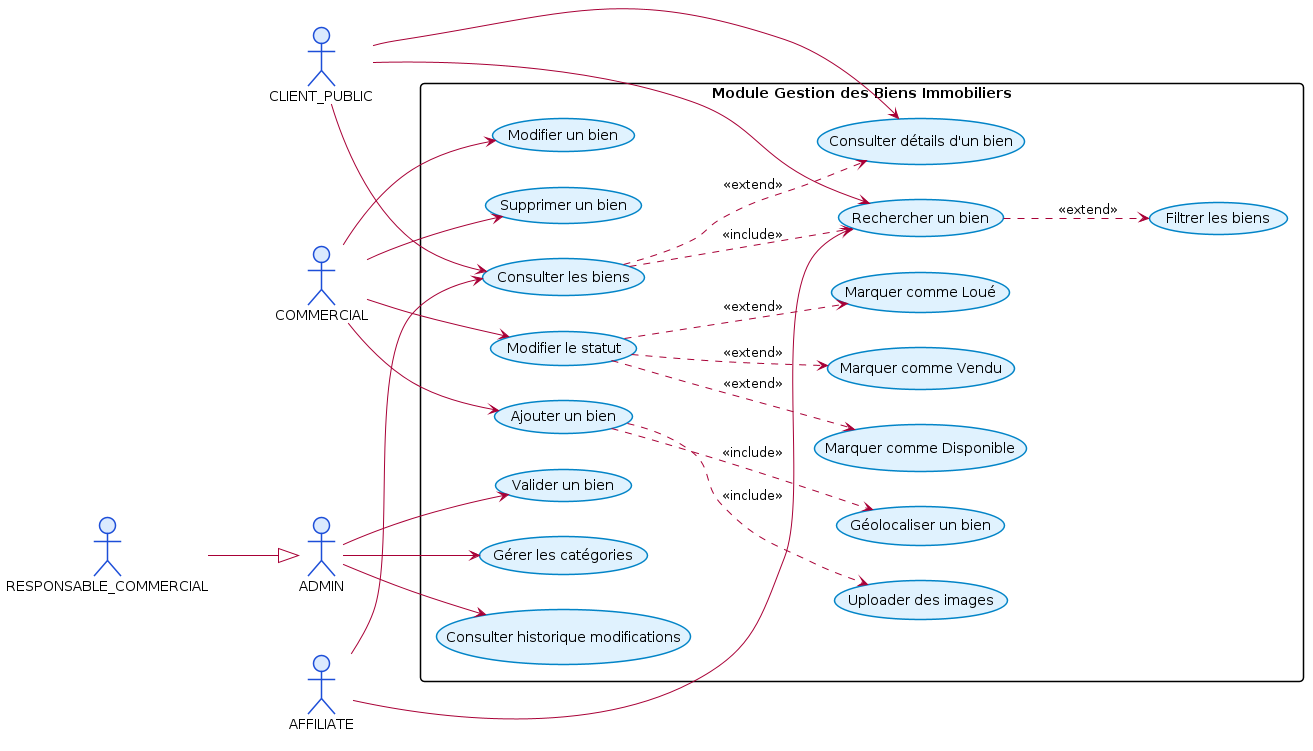
\includegraphics[width=0.88\textwidth]{images/usecase-biens.png}
}{%
    \fbox{\begin{minipage}{0.9\textwidth}
    \centering
    \vspace{4cm}
    \textit{[Diagramme de cas d'utilisation — Gestion des Biens]}
    \vspace{4cm}
    \end{minipage}}
}
\caption{Diagramme de cas d'utilisation du module Gestion des Biens Immobiliers}
\end{figure}

% ==================================================
% 10.4 DIAGRAMME DE CLASSES
% ==================================================

\subsection{Diagramme de classes}

Le diagramme de classes constitue le modèle structurel central de l'application. Il représente l'ensemble des entités du domaine, leurs attributs, leurs méthodes et les relations qui les unissent. Ce diagramme sert de base à la conception du schéma de la base de données MySQL ainsi qu'à la définition des entités JPA du backend Spring Boot.

Les principales entités identifiées sont les suivantes :

\begin{itemize}
    \item \textbf{User :} Entité centrale représentant tous les utilisateurs du système. Elle porte le rôle (\texttt{RoleType}), les informations personnelles et la relation hiérarchique parent-enfant.
    \item \textbf{Agency :} Représente une agence immobilière avec ses informations et son statut d'approbation.
    \item \textbf{Property :} Entité cœur du domaine immobilier, portant toutes les caractéristiques du bien, son statut et les indicateurs financiers.
    \item \textbf{Transaction / Contract :} Gèrent les opérations commerciales (ventes, locations) et leurs contrats associés.
    \item \textbf{Message / Conversation :} Supportent la messagerie interne temps réel.
    \item \textbf{AffiliateProfile / SaleOffer / Commission :} Modélisent le module affilié avec ses offres et commissions.
\end{itemize}

\begin{figure}[H]
\centering
\IfFileExists{images/class-diagram.png}{%
    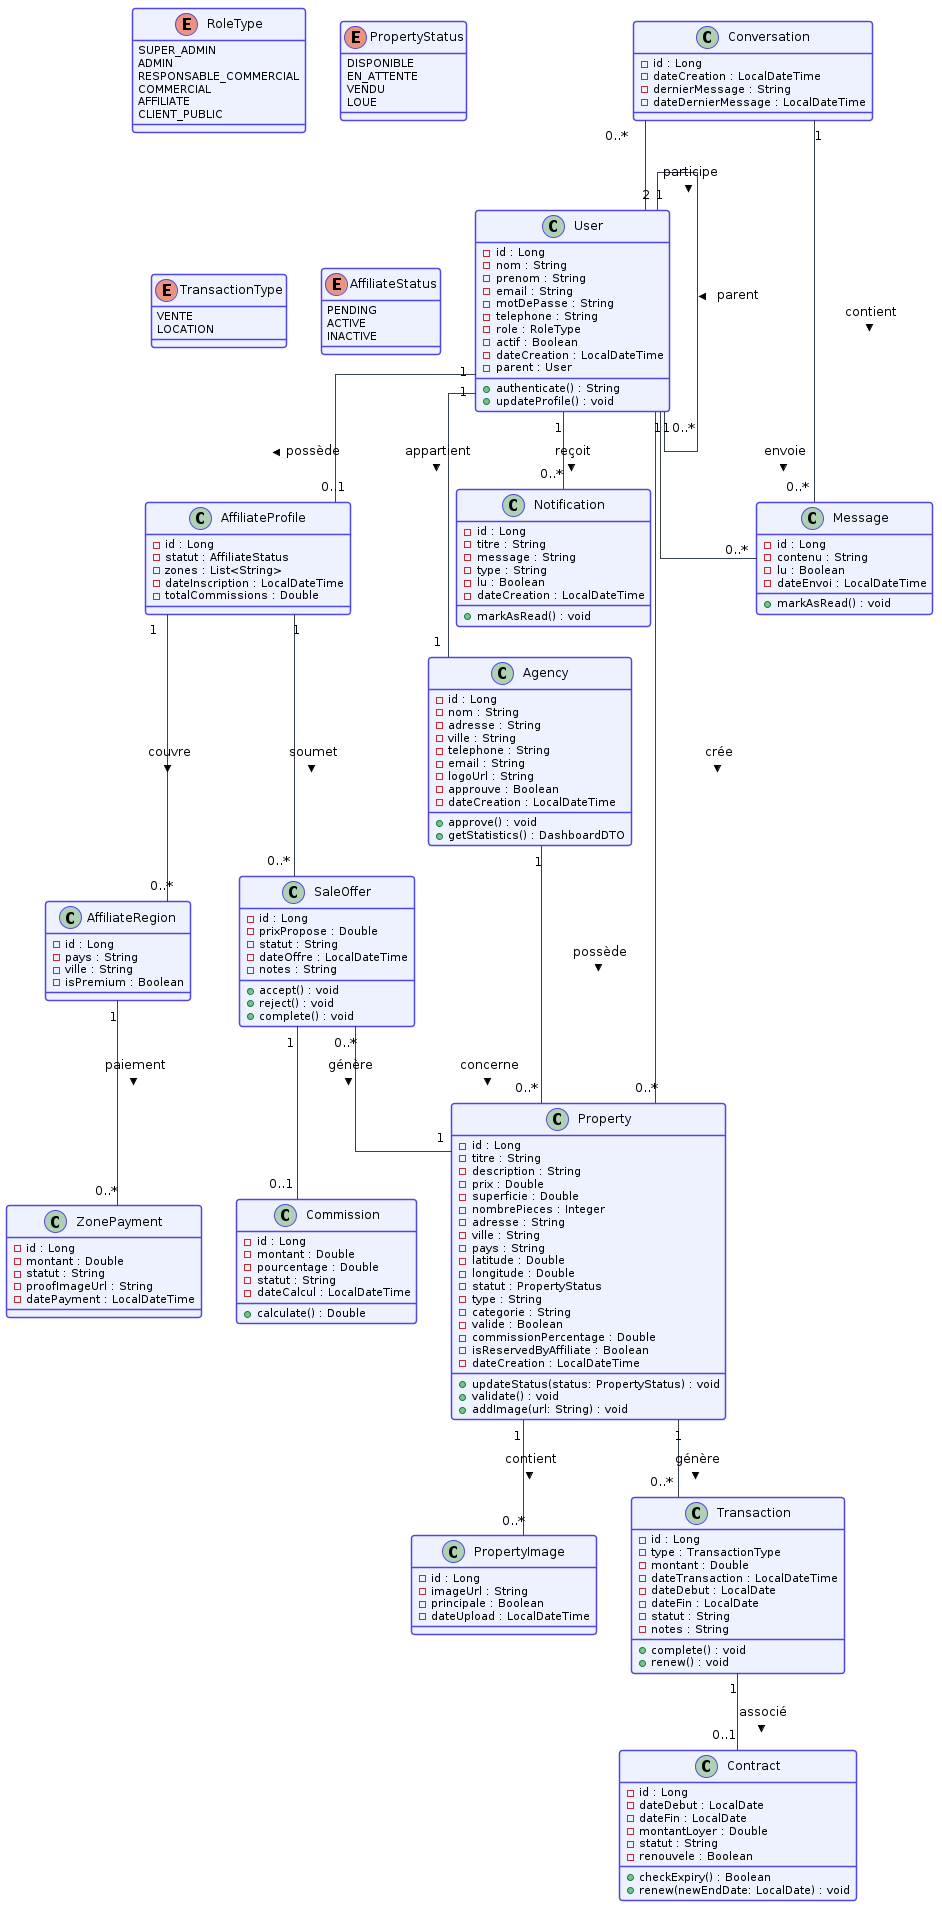
\includegraphics[width=0.97\textwidth]{images/class-diagram.png}
}{%
    \fbox{\begin{minipage}{0.9\textwidth}
    \centering
    \vspace{6cm}
    \textit{[Diagramme de classes]}
    \vspace{6cm}
    \end{minipage}}
}
\caption{Diagramme de classes de la plateforme Maison3D Immobilier}
\end{figure}

% ==================================================
% 10.5 DIAGRAMME DE SÉQUENCE - AUTHENTIFICATION
% ==================================================

\subsection{Diagramme de séquence — Authentification JWT}

Ce diagramme de séquence illustre le processus complet d'authentification d'un utilisateur sur la plateforme. Il décrit les interactions entre le navigateur (Angular), le contrôleur d'authentification (Spring Boot), le service de gestion des utilisateurs et le service JWT, jusqu'à la génération et au stockage du token.

\begin{figure}[H]
\centering
\IfFileExists{images/sequence-auth.png}{%
    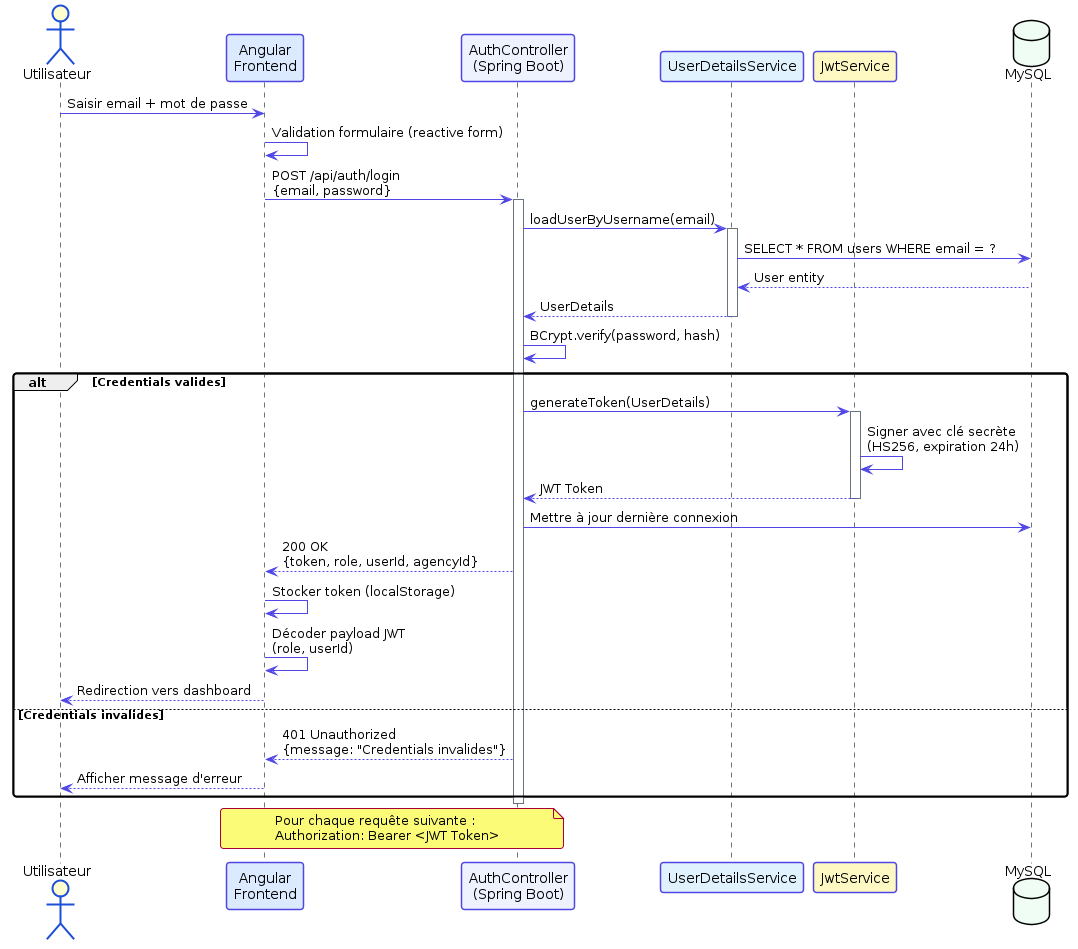
\includegraphics[width=0.90\textwidth]{images/sequence-auth.png}
}{%
    \fbox{\begin{minipage}{0.9\textwidth}
    \centering
    \vspace{4cm}
    \textit{[Diagramme de séquence — Authentification JWT]}
    \vspace{4cm}
    \end{minipage}}
}
\caption{Diagramme de séquence du processus d'authentification JWT}
\end{figure}

% ==================================================
% 10.6 DIAGRAMME DE SÉQUENCE - CHANGEMENT DE STATUT
% ==================================================

\subsection{Diagramme de séquence — Changement de statut d'un bien}

Ce diagramme de séquence modélise le processus de changement de statut d'un bien immobilier, en particulier lors du passage au statut VENDU ou LOUÉ. Il illustre la création automatique d'une transaction, la génération du contrat de location (si applicable) et l'envoi des notifications aux parties concernées.

\begin{figure}[H]
\centering
\IfFileExists{images/sequence-status-bien.png}{%
    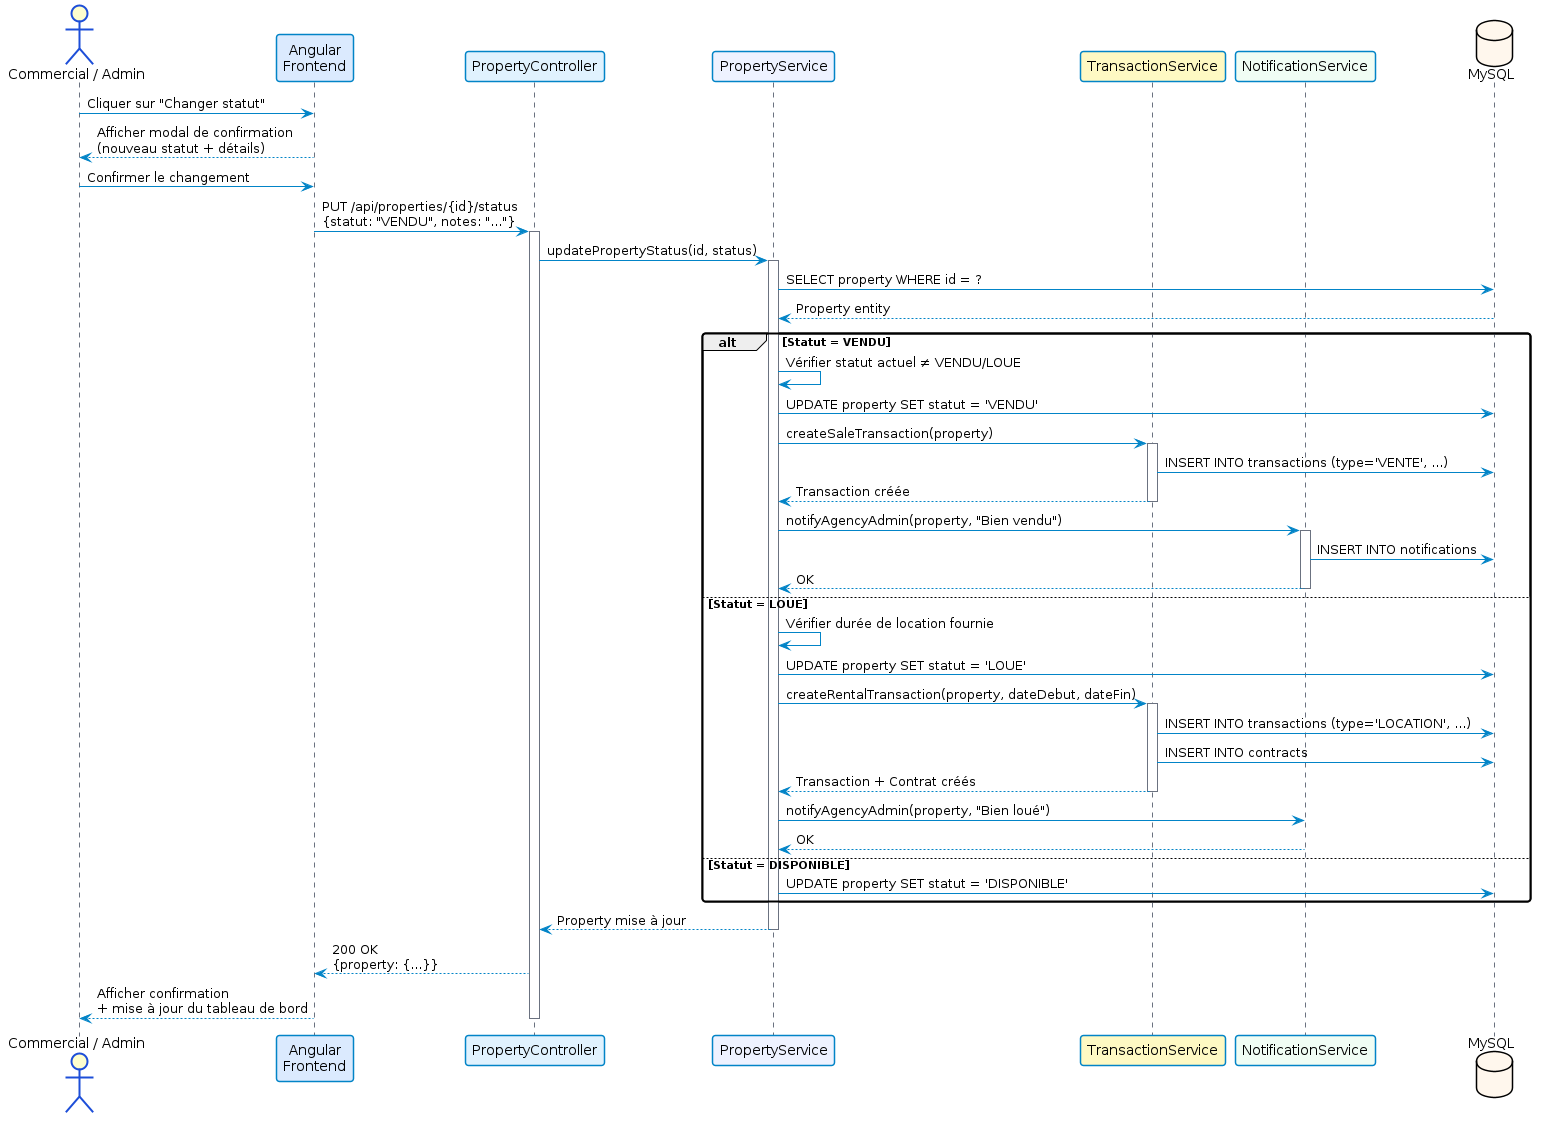
\includegraphics[width=0.90\textwidth]{images/sequence-status-bien.png}
}{%
    \fbox{\begin{minipage}{0.9\textwidth}
    \centering
    \vspace{4cm}
    \textit{[Diagramme de séquence — Changement de statut d'un bien]}
    \vspace{4cm}
    \end{minipage}}
}
\caption{Diagramme de séquence du processus de changement de statut d'un bien immobilier}
\end{figure}

% ==================================================
% 10.7 DIAGRAMME DE SÉQUENCE - AFFILIÉ
% ==================================================

\subsection{Diagramme de séquence — Cycle de vie d'une offre affilié}

Ce diagramme de séquence présente le cycle de vie complet d'une offre soumise par un affilié, depuis la consultation du catalogue personnalisé jusqu'au calcul et à la notification de la commission, en passant par la soumission et l'acceptation de l'offre.

\begin{figure}[H]
\centering
\IfFileExists{images/sequence-affiliate.png}{%
    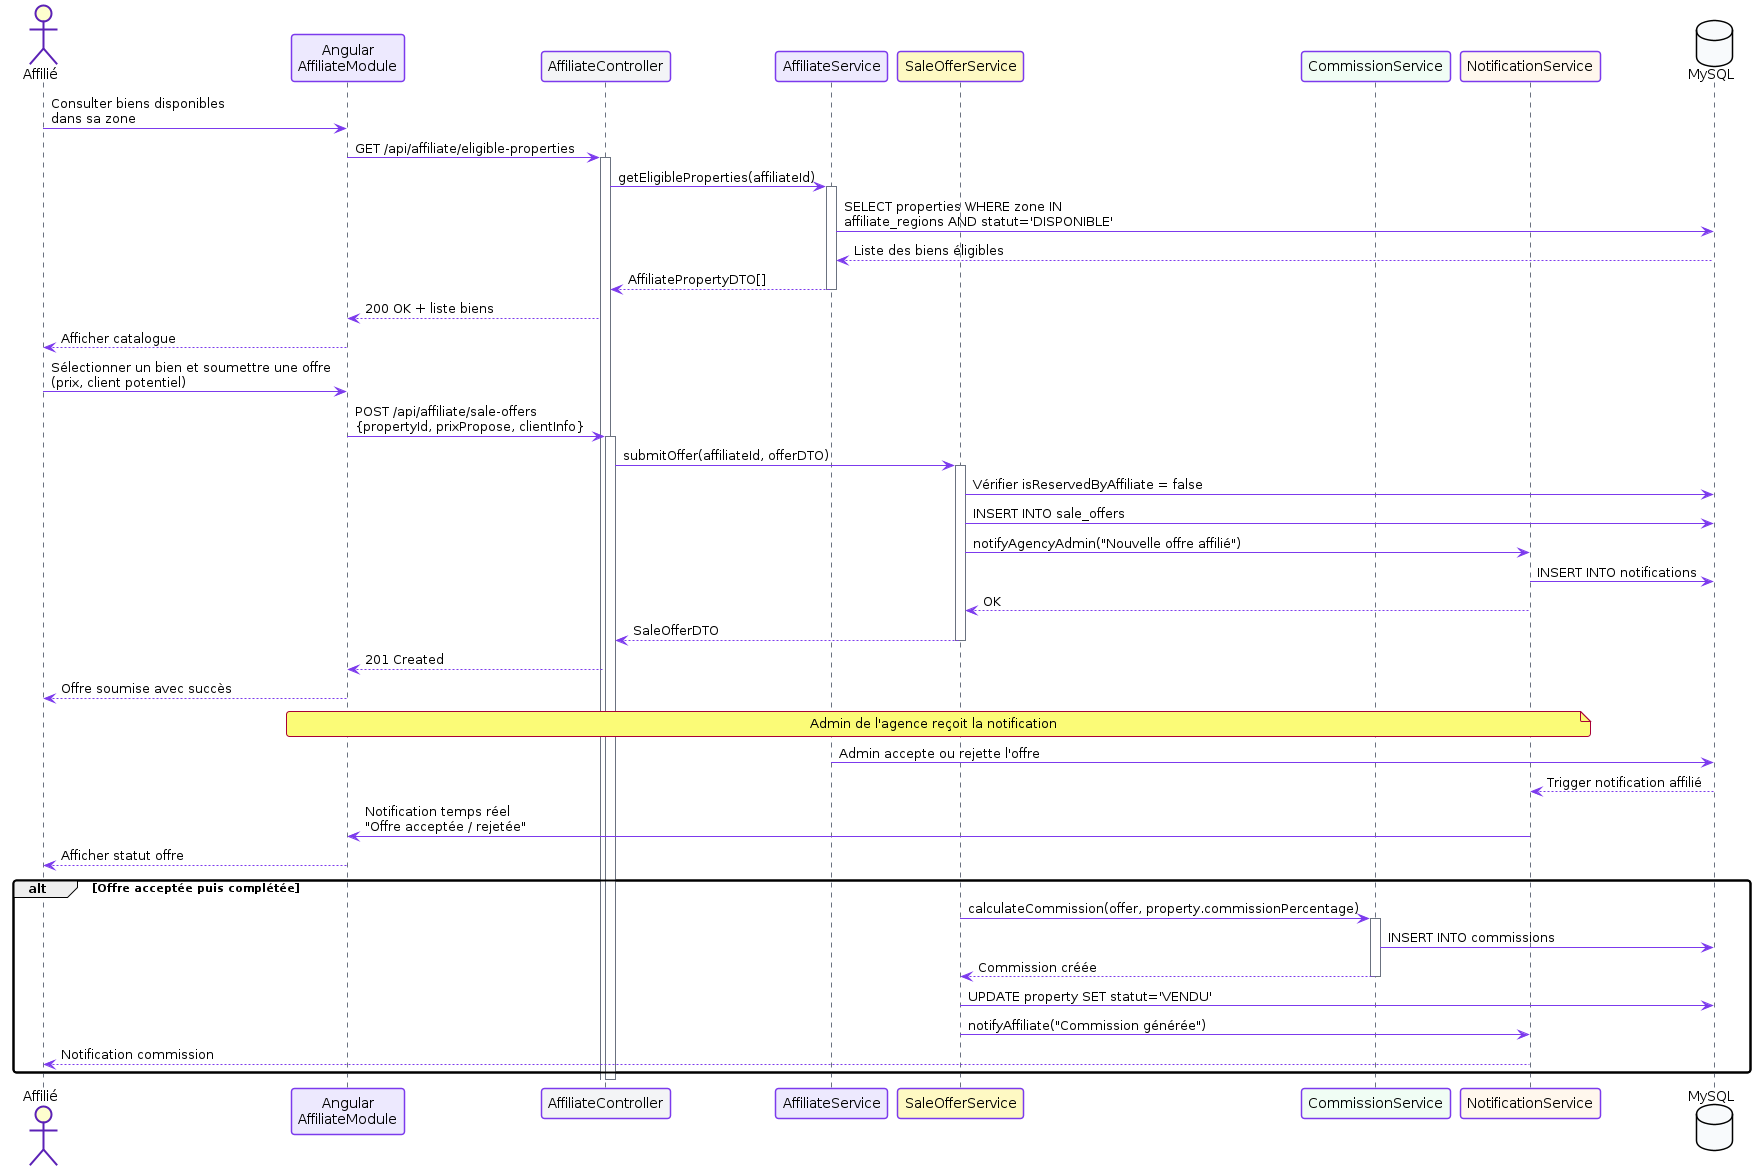
\includegraphics[width=0.90\textwidth]{images/sequence-affiliate.png}
}{%
    \fbox{\begin{minipage}{0.9\textwidth}
    \centering
    \vspace{4cm}
    \textit{[Diagramme de séquence — Cycle de vie d'une offre affilié]}
    \vspace{4cm}
    \end{minipage}}
}
\caption{Diagramme de séquence du cycle de vie d'une offre soumise par un affilié}
\end{figure}

% ==================================================
% 10.8 DIAGRAMME D'ACTIVITÉS
% ==================================================

\subsection{Diagramme d'activités — Ajout et validation d'un bien immobilier}

Le diagramme d'activités suivant modélise le processus complet d'ajout et de validation d'un bien immobilier, depuis la saisie des informations par le commercial jusqu'à la publication du bien sur le portail public après validation par l'administrateur. Il met en évidence les points de décision et les alternatives du processus.

\begin{figure}[H]
\centering
\IfFileExists{images/activity-ajout-bien.png}{%
    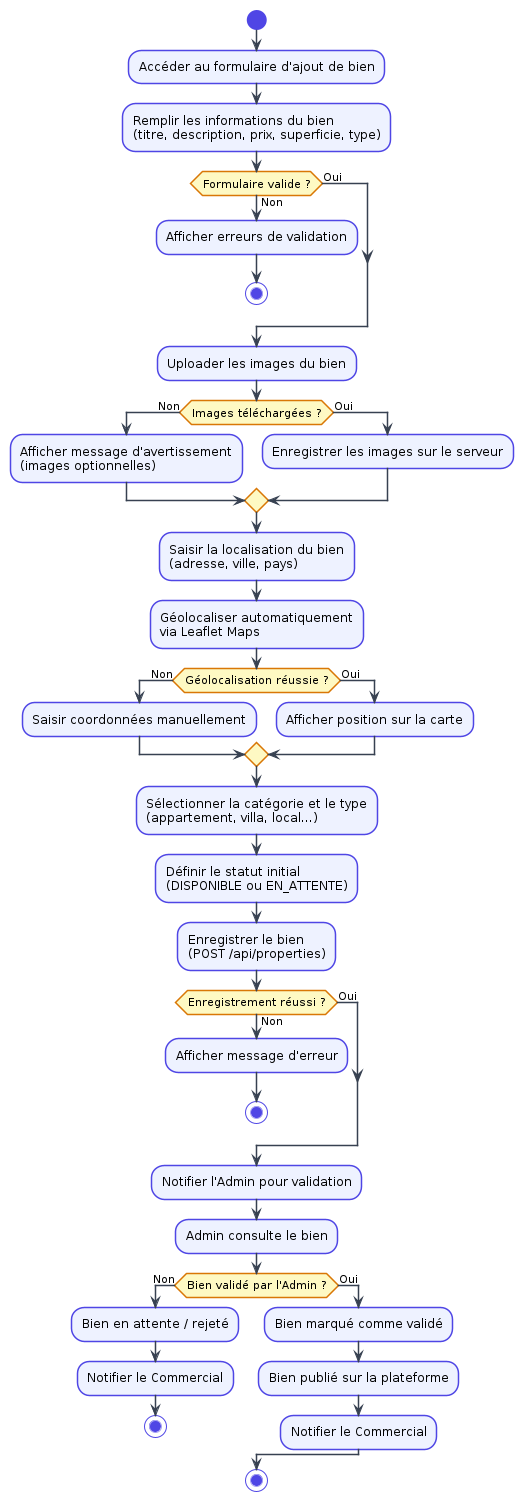
\includegraphics[width=0.75\textwidth]{images/activity-ajout-bien.png}
}{%
    \fbox{\begin{minipage}{0.9\textwidth}
    \centering
    \vspace{4cm}
    \textit{[Diagramme d'activités — Ajout d'un bien immobilier]}
    \vspace{4cm}
    \end{minipage}}
}
\caption{Diagramme d'activités du processus d'ajout et de validation d'un bien immobilier}
\end{figure}

% ==================================================
% 10.9 DIAGRAMME DE DÉPLOIEMENT
% ==================================================

\subsection{Diagramme de déploiement}

Le diagramme de déploiement illustre l'architecture physique de la plateforme, en représentant les nœuds matériels et logiciels impliqués dans le déploiement de l'application. Il présente les conteneurs Docker, les serveurs, les connexions réseau et les services externes utilisés par la plateforme.

\begin{figure}[H]
\centering
\IfFileExists{images/deployment.png}{%
    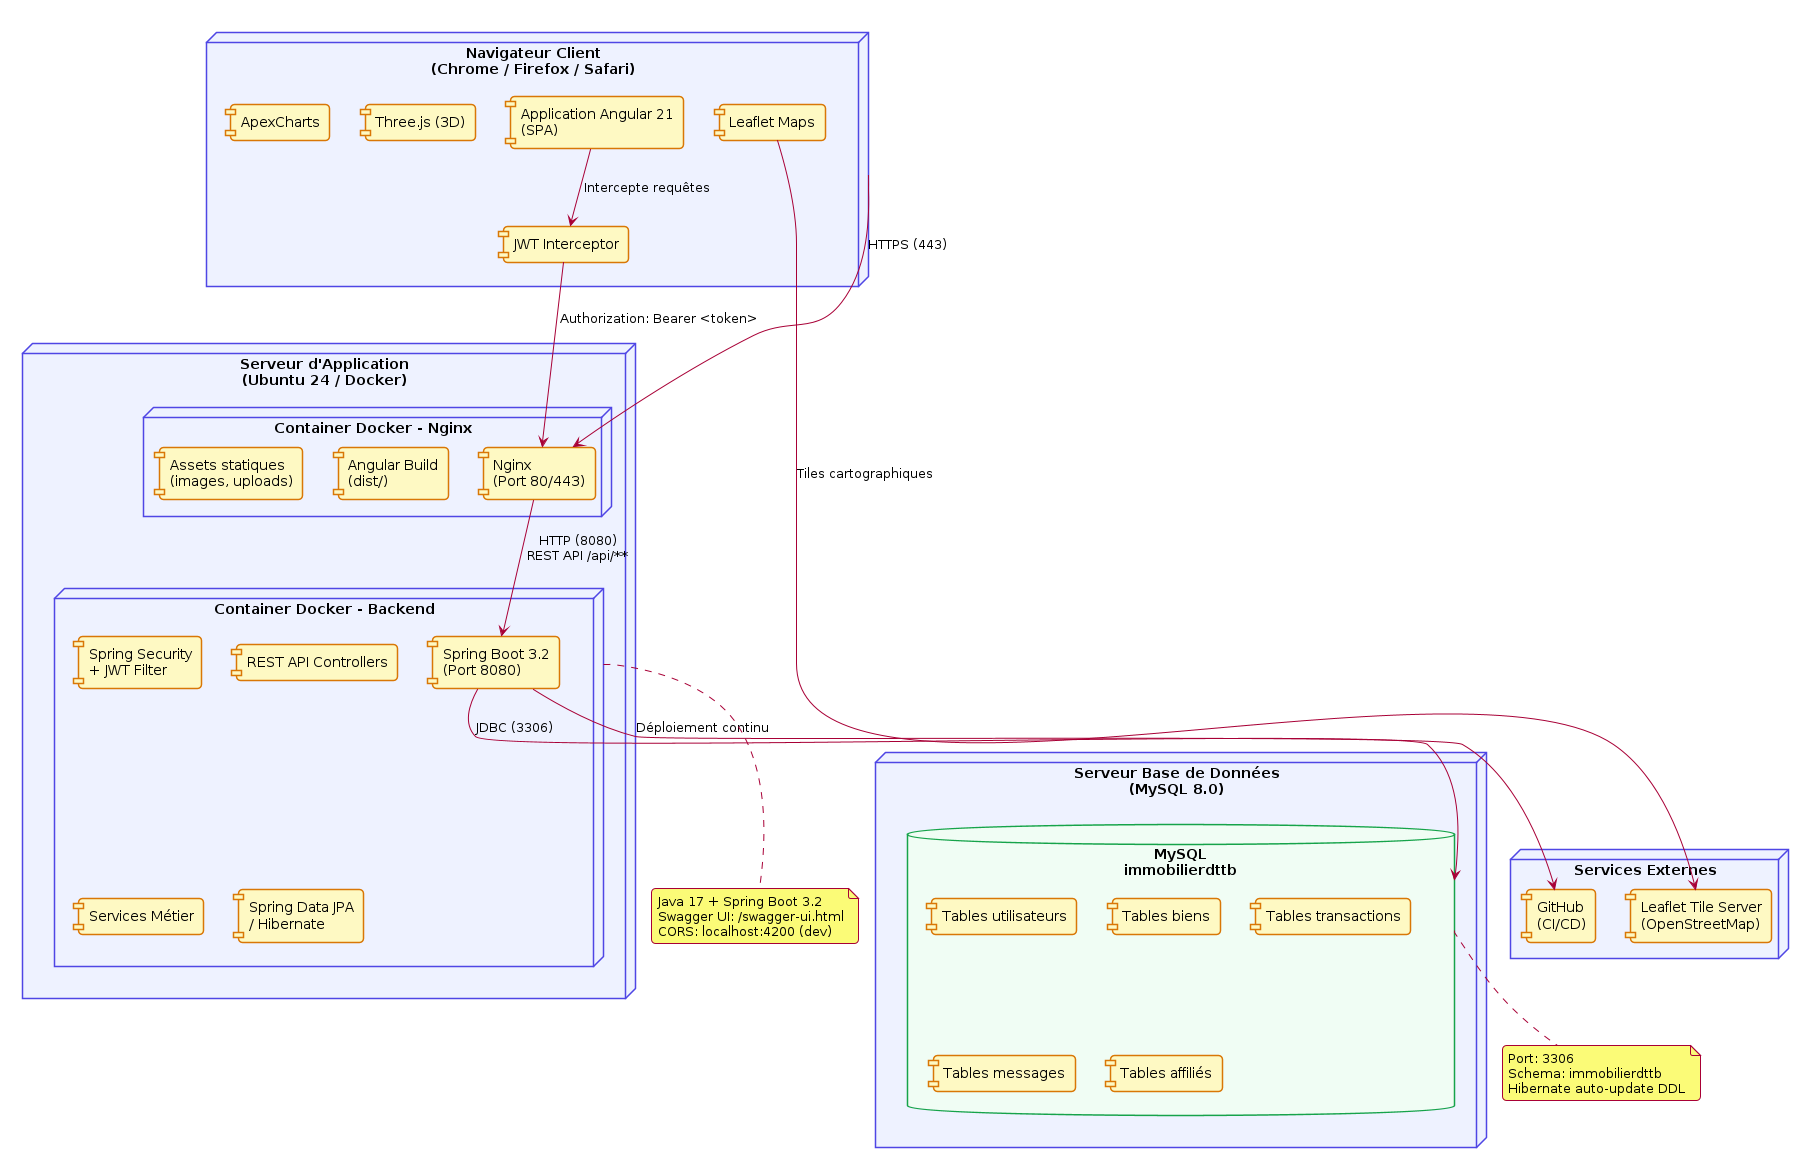
\includegraphics[width=0.92\textwidth]{images/deployment.png}
}{%
    \fbox{\begin{minipage}{0.9\textwidth}
    \centering
    \vspace{4cm}
    \textit{[Diagramme de déploiement]}
    \vspace{4cm}
    \end{minipage}}
}
\caption{Diagramme de déploiement de la plateforme Maison3D Immobilier}
\end{figure}

% ==================================================
% 10.10 DIAGRAMME DE COMPOSANTS
% ==================================================

\subsection{Diagramme de composants}

Le diagramme de composants présente l'organisation modulaire de l'application en illustrant les composants logiciels, leurs interfaces et leurs dépendances. Il met en évidence la séparation entre les modules Angular (frontend), les contrôleurs et services Spring Boot (backend) et les repositories d'accès aux données.

\begin{figure}[H]
\centering
\IfFileExists{images/component-diagram.png}{%
    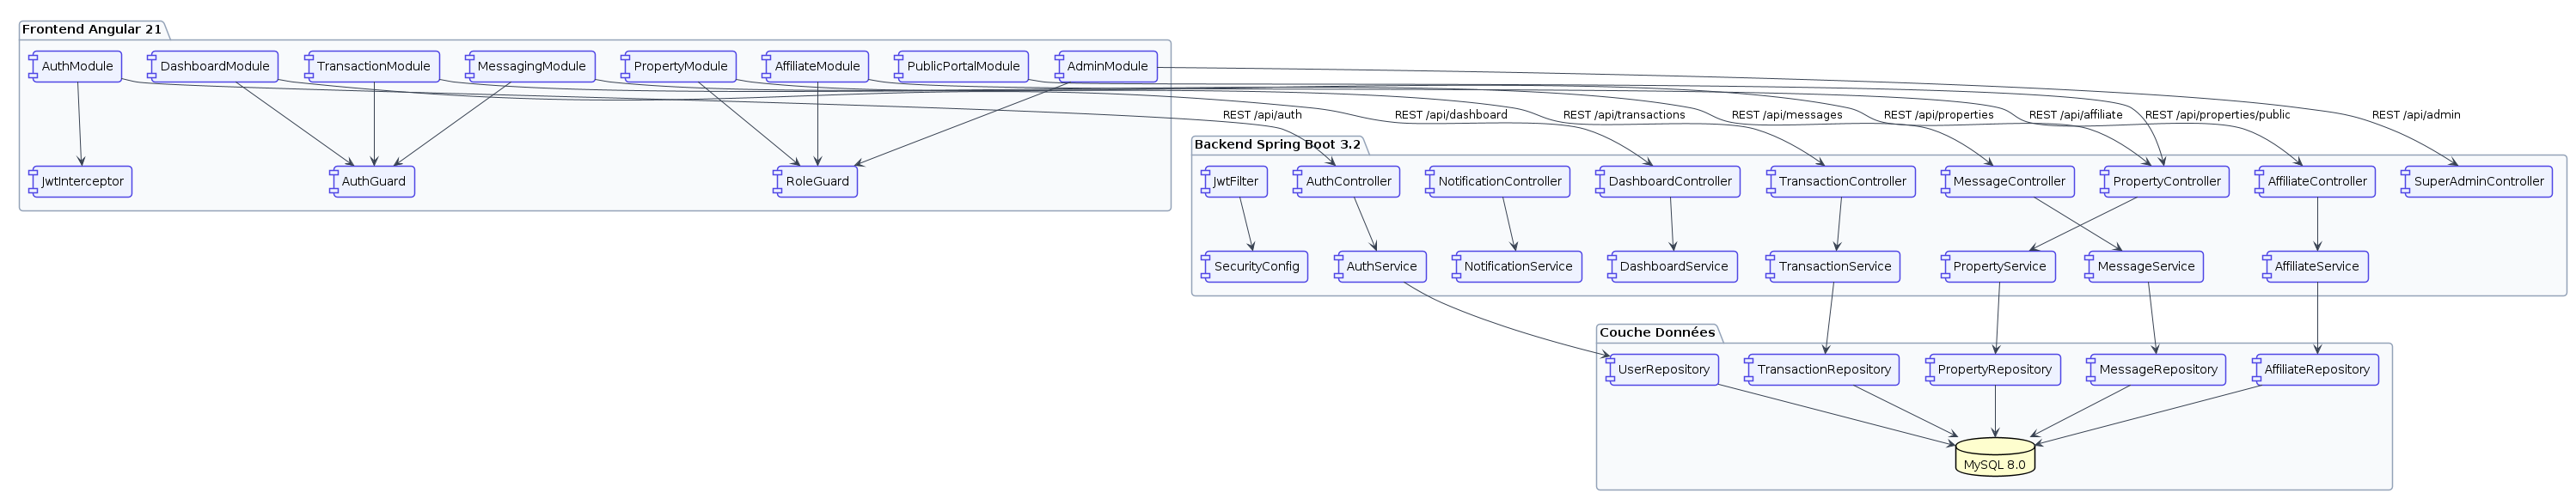
\includegraphics[width=0.95\textwidth]{images/component-diagram.png}
}{%
    \fbox{\begin{minipage}{0.9\textwidth}
    \centering
    \vspace{4cm}
    \textit{[Diagramme de composants]}
    \vspace{4cm}
    \end{minipage}}
}
\caption{Diagramme de composants de la plateforme Maison3D Immobilier}
\end{figure}

% ==================================================
% SECTION 11 : CONCLUSION
% ==================================================

\section{Conclusion}

Ce chapitre a permis de poser les fondations techniques et analytiques du projet \textbf{Maison3D Immobilier}. À travers une démarche structurée et rigoureuse, nous avons défini avec précision les objectifs stratégiques et opérationnels de la plateforme, identifié et décrit en détail les six acteurs du système, et dressé un inventaire complet des besoins fonctionnels organisés par modules. Nous avons également précisé les exigences non fonctionnelles en termes de sécurité, de performance, d'ergonomie et de maintenabilité.

L'architecture générale de la plateforme, fondée sur le modèle 3-Tiers, a été présentée et justifiée, et les choix technologiques retenus — Angular 21, Spring Boot 3.2, MySQL 8.0 et JWT — ont été argumentés en regard des besoins du projet. Enfin, une modélisation UML complète a été réalisée, couvrant les dimensions statiques (diagramme de classes, composants) et dynamiques (diagrammes de séquence, d'activités) du système, ainsi que les perspectives de déploiement.

Ces éléments d'analyse et de conception constituent la référence technique qui guidera l'ensemble des sprints de développement présentés dans les chapitres suivants. Le prochain chapitre sera consacré à la réalisation du premier sprint, portant sur les modules fondamentaux d'authentification et de gestion des agences.

\end{document}